%\documentclass[12pt,preprint]{aastex}
%\documentclass[preprint2,12pt]{aastex}
\documentclass{emulateapj}
%\usepackage{apjfonts}
\usepackage{graphicx}
\usepackage{amssymb}
\usepackage{amsmath}
\usepackage{todonotes}

\shortauthors{LGB, KM, JNW}
\shorttitle{Toy transit surveys}

\begin{document}

% ------------------------------------------------------------------------
% New commands
%
\def\ltsima{$\; \buildrel < \over \sim \;$}
\def\lsim{\lower.5ex\hbox{\ltsima}}
\def\gtsima{$\; \buildrel > \over \sim \;$}
\def\gsim{\lower.5ex\hbox{\gtsima}}
\def\tess{{\it TESS} }
\def \teff {T_{\rm eff}}
\def \phir {\Phi_{\rm R}}
\def \fov {24$^{\circ}$}
\def \pixsz {21.1''}
\def \aeff {69.1 cm$^2$ }    
\def \epd {105 mm}                          

\def \kepler {{\it Kepler}}

% -------------------------------------------------------------------------
%

\bibliographystyle{apj}

\title{ Toy Transit Surveys }

\author{
  LGB, KM, JNW
}

% \journalinfo{Draft version}
\slugcomment{Memo for internal use}

%\altaffiltext{1}{Princeton University}

\begin{abstract}

What errors does ignoring binarity introduce on the occurrence rates derived 
from transit surveys?

First, we show that in a universe where all stars have fixed properties
(except that some are twin binaries), the results of a search for planets of a 
given radius and orbital period can be expressed analytically.

Then, we allow the properties of the secondary in binary systems to vary. A 
distribution of light ratios introduces a heavy detection bias towards 
equal-mass binaries in magnitude limited samples.
We show that dependent upon planet occurrence's functional dependence on host 
star mass (and binarity), the errors introduced in derived occurrence rates vs. 
real occurrence rates can range from a few percent to at most $\approx 60\%$ 
relative error.

Finally, we perform a synthetic transit survey analogous to {\it Kepler}. We 
show that if we assume every star in this {\it Kepler} survey analog is single, 
we underestimate occurrence rates for a given planet radius and period by 
$\approx 39\%$.
This is immediately applicable to the question of Earth-like planets around 
Sun-like stars.


\end{abstract}

\keywords{planets and satellites:\ detection}

\section{Introduction}

Ah, transiting planets! We learn so much by studying them. But how much can we 
actually learn, and how much is messed up by binarity?

Binary companions to single stars introduce a surprising number of biases into 
transit surveys.
For a start, any magnitude limited survey over-represents binaries compared to 
a volume-limited survey -- the familiar Malmquist bias, though in a slightly 
different context.
While transit surveys are ideally signal to noise limited, if the noise 
properties of the survey are dominated by photon counting noise, a signal to 
noise limit becomes equivalent to a magnitude limit.
Thus stars surveyed in transit surveys must also over-represent binaries 
compared to those in a volume-limited sample.

A more straight-forward effect of binarity on transit surveys is that any star 
which is unknowingly a double introduces extra stars about which planets might 
be detectable.
However, this apparent increase in the number of searchable stars is mitigated 
by dilution: the observed transit depths in such systems are reduced by 
contaminating flux from the binary companion. This dilution is especially 
drastic if the planet orbits the secondary, in which case dilution impacts 
detectability the most.

A related effect to dilution is misinterpretation of transit depths. If the 
planet to star radius ratio is directly taken as the square-root of 
the observed transit depth, derived planetary radii in binary systems will 
systematically too small.
Ciardi et al [2015] explored this issue in depth. They showed that for the case 
of \kepler, assuming host stars to always be single will on 
average underestimate radii by a multiplicative factor of $\approx 1.5$.

Finally, binarity may affect transit surveys through actual astrophysics.
For the relatively rare case [Duquennoy \& Mayor 1991, Raghavan et al 2010] of 
close binaries, dynamical stability imposes a limited range of periods in which 
planets may orbit [e.g., Holman \& Weigert 
1999, Li et al 2017], the effects of which have been observed [Kraus et al 
2016].
Also, the formation rates of planets, and thus their intrinsic occurrence 
rates, may be influenced by properties of circumprimary and/or circumbinary 
disks.
Although the observations are still ongoing, early results seem to indicate 
that once binary companions are $\gtrsim 100\,{\rm AU}$ apart, binarity does 
not decrease planet occurrence rates [CITE], and may even increase them for 
giant planets [Ngo et al 2017].

\section{Model \#1: fixed stars, fixed planets, fixed light-ratio binaries}
\label{sec:model_1}

Binarity introduces several convoluted effects on transit 
surveys. To disentangle them, imagine the following idealized survey:

\begin{enumerate}
\item You are going to observe the entire sky for a duration $T_{\rm obs}$, 
with a detector of area $A$, and known bandpass. Your detector is photon-noise 
limited.
%
\item You are interested only in detecting planets of radius $R_p$, and orbital 
period $P$. For instance, $R_p=R_\oplus$, $P={\rm 1\ year}$.
%
\item You are only interested in detecting them around stars of radius $R_1$, 
and luminosity $L_1$. For instance, G2V dwarfs.
%
\item You can only detect your `nominal planet' when you observe signals with
${\rm S/N} > {\rm (S/N)_{min}}$.
For a photon-noise limited survey, this minimum signal to noise ratio is 
equivalent to a minimum flux, $F_{\rm min}$.
%
\item However, you opt to observe all the ``points'' on-sky with apparent 
magnitude $m < m_{\rm lim}$, or equivalently with energy flux in your bandpass 
greater than some limit $F > F_{\rm lim}$.
(You will not be able to detect planets around the faintest of 
these, and will need to perform a completeness correction to later derive 
occurrence rates.)
Generally $F_{\rm lim} < F_{\rm min}$, \textit{e.g.}, whenever the original 
magnitude cut defines a ``source catalog'' from which ``searchable stars'' are 
selected, as in the KIC [Batalha et al, 2010, Brown et al 2011] and the TIC 
[Stassun et al 2017].
\end{enumerate}

You get funding, and perform the S/N-limited survey. All planets with 
${\rm S/N} > {\rm (S/N)_{min}}$ are detected. The rest are not.
You now wish to derive an occurrence rate for planets of radius $R_p$ and 
orbital period $P$.
Assume your universe is a universe in which:
\begin{itemize}
	\item The true population of ``points'' (stellar systems, all unresolved) 
	comprises both single and double star systems. Single star systems have 
	luminosity in the observed bandpass $L_1$, radii $R_1$, and effective 
	temperature $T_{\rm eff,1}$.
	Double star systems have luminosity in the observed bandpass $L_d = 
	(1+\gamma_R)L_1$, for $\gamma_R = L_2/L_1$ the ratio of the luminosity of 
	the secondary to the primary. 
	In this section, $\gamma_R$ is a constant across the population 
	of star systems.
	The ratio of the two number densities in a 
	volume-limited sample is the binary fraction\footnote{The binary fraction 
		is equivalent to the multiplicity fraction if there are no triple, 
		quadruple, $\ldots$ systems.}.
	\item The true population of planets around these stars is as follows:
	\subitem A fraction $\Gamma_{t,s}$ of stars in single star systems 
	have a planet of radius $R_p$, with orbital period $P$.
	\subitem A fraction $\Gamma_{t,d}$ of each star in a double star 
	system has a planet of radius $R_p$, with orbital period $P$. For instance, 
	if $\Gamma_{t,s} = \Gamma_{t,d} = 0.1$, on average each double 
	system contributes 0.2 planets, and each single system 0.1 planets.
	Any astrophysical difference in planet formation between singles and 
	binaries is captured by these two terms.
	Note that we are taking an limit by assuming the primary and secondary of 
	a binary system host planets at equal rates. If the secondary is 
	non-identical to the primary, it's clearly wrong.	
\end{itemize}



For simplicity, one might wish to imagine the observer correctly 
pre-selects all of the ``searchable stars'', in the style of [Pepper et al, 
2003].
In other words, they would begin by knowing ${\rm (S/N)_{min}}$, and then only 
observe stars for which they would have adequate flux to achieve it -- setting 
$F_{\rm lim} = F_{\rm min}$.
This simplification would naively allow the observer to ignore 
completeness effects when deriving occurrence rates, since their completeness 
is 100\%.

We do not begin this way because in a stellar population of both singles and 
binaries, the above approach ignores necessary incompleteness for 
binary systems.
If we set the limiting flux to give 100\% completeness for single stars, we 
will unwittingly select binaries near that flux limit, for which dilution 
will push transit signals below the detection threshold.
This is because a flux limit maps onto three different maximum 
detection distances for a population of single stars and twin binaries:
\begin{enumerate}
\item $d_{{\rm max},s}$: the maximum distance out to which single stars are
  selected. This can be chosen to coincide with the maximum distance out to
  which planets are detectable around single stars.
%
\item $d_{{\rm max},d}^\star$: the maximum distance out to which double stars
  are selected. This is different from $d_{{\rm max},d}^{\rm p}$, the maximum
  distance out to which planets are detectable around double stars. For a 
  population with fixed  $\gamma_R$, since ${\rm S/N} \propto \mathcal{D} 
  L^{-1/2} d$,
  \begin{equation}
    d_{{\rm max},d}^{\rm p} = (1 + \gamma_R)^{-1/2} d_{{\rm max},s} = 
    (1 + \gamma_R)^{-1} d_{{\rm max},d}^\star.
  \end{equation}
  For $\gamma_R = 1$, this means only 1 in 8 selected binary stars can yield
  detectable planets.
\end{enumerate}
We develop tools to address this and related completeness effects from the 
outset.


Consider the following questions:
\begin{enumerate}
\item How many single and double star systems, respectively, are in the sample?
Correspondingly, how many stars are in the sample?

\item How many planets are in the sample? (Orbiting single stars, and orbiting 
double stars respectively).

\item What is the true occurrence rate?

\item How many planets are detected?

\item What occurrence rate does astronomer A, who has never heard of binary 
star systems, or completeness, derive for planets of radius $R_p$ and period 
$P$?

\item What occurrence rate does astronomer B, who accounts for the ``2 for 1'' 
effect of binarity (\textit{i.e.} that the sample actually has more stars than 
astronomer A thought) derive? (Astronomer B neglects completeness).

\item What about astronomer C, who accounts for ``2 for 1'' \textit{and} 
misclassification due to diluted radii? In other words, astronomer C did a 
combination of high resolution imaging and RV followup on every candidate, and
correctly classifies the planetary radii in every case.

\item What about astronomer D, who additionally notes the importance of 
completeness?
\end{enumerate}


\subsection{How many stars are in the sample?}

Let $N_s$ be the number of single star systems, and $N_d$ the number of double 
star systems. Then the total number of stars in the sample is
\begin{equation}
N_{\rm stars} = N_s + 2N_d.
\end{equation}

In a magnitude-limited sample in which stars are uniformly distributed in 
volume, the number of stars will be the number density times the volume.
If the volume is taken to be a sphere over which the number density is uniform,
\begin{equation}
N_i = n_{i} \frac{4\pi}{3} d_{{\rm max},i}^3,
\label{eq:number_systems}
\end{equation}
for $i\in{\rm \{single,double\} } \equiv { \{s,d\} }$, and
\begin{equation}
\frac{n_{d}}{n_{s}} = {\rm binary\ fraction} \equiv {\rm BF}
\end{equation}
by definition. The absolute normalization of the number density is a measured 
quantity, as is the binary fraction. For G2V dwarfs, the latter is $\approx 
0.45$ [Duchene \& Kraus, 2013]. The former is given by [Bovy 2017].

$d_{{\rm max},i}$ in Eq.~\ref{eq:number_systems} is the maximum distance 
corresponding to the given magnitude limit:
\begin{equation}
d_{{\rm max},i} = \left(\frac{L_{i}}{4 \pi F_{{\rm min}}}\right)^{1/2},
\label{eq:d_max}
\end{equation}
where the limiting flux in the bandpass $F_{{\rm min}}$ can also be 
stated in terms of the limiting magnitude $m_{{\rm min}}$,
\begin{equation}
m_{{\rm min}} = m_{0} - \frac{5}{2} \log_{10} \left(\frac{F_{{\rm 
min}}}{F_{0}}\right),
\end{equation}
for $m_{0}$ a zero-point magnitude and $F_{0}$ its corresponding flux (as 
always, everything is implicitly written in a defined bandpass).

In Eq.~\ref{eq:d_max}, again $i\in{\rm \{single,double\} }$, and as a 
consequence the maximum distance to which binary stars will be selected is 
greater than that of single stars, simply as a consequence of imposing a 
magnitude cut.
The ratio of double to single systems is
\begin{align}
\frac{N_d}{N_s} &= 
	\frac{n_d}{n_s} \left(\frac{d_{{\rm max}, d} }{d_{{\rm max}, s}}\right)^3 \\
&= {\rm BF} \times (1+\gamma_R)^{3/2}.
\end{align}
In the nominal case of twin binaries ($\gamma_R = 1$), with a binary fraction 
${\rm BF} = 0.5$, there are 
$\sqrt{2}$ more binary systems than single systems in the sample.
Correspondingly, there are $2\sqrt{2}$ more stars in binary systems than stars 
in single systems.

As a comment on Eq.~\ref{eq:number_systems}, if 
we wished to write a stellar number density profile that accounted for the 
vertical structure of the Milky Way, we might choose a profile either 
$\propto \exp(-z/H)$, or $\propto {\rm sech}^2(z/H)$ for $z$ the distance from 
the galactic midplane and $H$ a scale-height. Both density profiles would lead 
closed form analytic solutions.



\subsection{How many planets are in the sample?}

The number of planets in the sample is
\begin{align}
N_{\rm planets} =& N_{\rm planets\ in\ single\ star\ systems}  +  \\
				  &\quad\quad N_{\rm planets\ in\ double\ star\ systems} 
				  \nonumber \\
			   =& \Gamma_{t,s} N_s + 2 \Gamma_{t,d} N_d.
\end{align}

The factor of 2 accounts for the fact that there are twice as many stars in 
double star systems.



\subsection{What is the true occurrence rate?}
\label{sec:true_rate}

The ``true occurrence rate'' is the average number of planets per star. Thus

\begin{align}
\Gamma_t &= \frac{N_{\rm planets}}{N_{\rm stars}} \\
\Gamma_t &= \frac{\Gamma_{t,s} N_s + 2 \Gamma_{t,d} N_d}{N_s + 2N_d}.
\label{eq:true_occ}
\end{align}



\subsection{How many planets are detected?}
The total number of planet detections is the sum of the number of planets 
detected in single star systems $N_{{\rm det},s}$ and the number of planets 
detected in double star systems $N_{{\rm det},d}$.
These can be expressed individually. 
The former is
\begin{equation}
N_{{\rm det},s} = N_s \Gamma_{t,s} f_{s,{\rm geom}} f_{s,{\rm S/N} > {\rm 
(S/N)_{min}}},
\label{eq:N_det_s}
\end{equation}
where the product $N_s \Gamma_{t,s}$ is the number of planets in the single 
star systems of the sample, $f_{s,{\rm geom}}\equiv f_{s,g}$ is the geometric 
transit probability, and $f_{s,({\rm S/N} > {\rm (S/N)_{min}})} \equiv f_{s,c}$ 
is the fraction of these transiting planets that are observed with signal to 
noise greater than the minimum detection threshold (the completeness). 
Analogously,
\begin{equation}
N_{{\rm det},d} = 2 N_d \Gamma_{t,d} f_{d,g} f_{d,c},
\label{eq:N_det_d}
\end{equation}
where now $2 N_d \Gamma_{t,d}$ is the number of planets in the double star 
systems of the sample, the geometric transit probability is the same (if we 
have twin binaries -- not if we consider a distribution of secondaries) and the 
completeness term must account for any differences in the signal to noise 
distribution that come from stellar binarity.


\subsubsection{Analytic completeness}
Since the geometric transit probability is known, the only terms we have yet to 
compute are the completeness terms, $f_{i,c}$ for $i\in{\rm \{single,double\} 
}$. We proceed as follows.

The signal ${\rm S}$ for a box-car train transiting planet is
\begin{align}
{\rm S} &= \delta \mathcal{D} \\
&= \left(\frac{R_p}{R_\star}\right)^2 \mathcal{D},
\end{align}
for $R_p$ the planet's radius, $R_\star$ that of its host star, and 
$\mathcal{D}$ the dilution parameter defined as
\begin{align}
  \mathcal{D} &= 
  \Bigg\{\begin{array}{lr}
  L_1 / L_d, & {\rm\ if\ binary\ and\ target\ primary}\\
  \gamma_R L_1 / L_d, & {\rm\ if\ binary\ and\ target\ 
  secondary}\\
  1, & {\rm\ if\ single},
  \end{array} \nonumber\\
  &=
    \Bigg\{\begin{array}{lr}
    (1+\gamma_R)^{-1}, & {\rm\ if\ binary\ and\ target\ primary}\\
    (1 + \gamma_R^{-1})^{-1}, & {\rm\ if\ binary\ and\ target\ 
    	secondary}\\
    1, & {\rm\ if\ single},
    \end{array} 
  \label{eq:dilution}
\end{align}
where $L_1, L_d,$ and $\gamma_R$ were defined in the opening monograph.

Assuming the only source of noise is Poissonian counting noise, the noise ${\rm 
N}$ can be written
\begin{equation}
{\rm N} = \frac{1}{\sqrt{N_\gamma}},
\end{equation}
for $N_\gamma$ the number of photons received by the detector. This noise model 
is a useful simplification -- see [Howell 2006, pg 75] for the full 
CCD equation.
The number of received photons can be written
\begin{equation}
N_\gamma = F^{\rm N}_\gamma A N_{\rm tra} T_{\rm dur},
\end{equation}
for $F^{\rm N}_\gamma$ the photon number flux from the system [${\rm 
ph\,cm^{-2}\,s^{-1}}$], 
$A$ the detector area, $T_{\rm dur}$ the transit duration, and $N_{\rm tra} $ 
the number of transits observed, which is multiplied in assuming the transits 
are ``phase-folded''.
	
Thus the signal to noise ratio can be written
\begin{equation}
{\rm S/N} = \delta \mathcal{D} \sqrt{F^{\rm N}_\gamma A N_{\rm tra} T_{\rm 
dur}}.
\label{eq:snr_ivory_tower}
\end{equation}

This means we can write the minimum number flux of photons required for a 
detection at threshold as
\begin{equation}
F_{\rm lim}^N = \left[ \left({\rm \frac{S}{N}}\right)_{\rm min} \frac{1}{\delta 
	\mathcal{D}} \right]^2 \frac{1}{A N_{\rm tra} T_{\rm dur}}.
\end{equation}
To convert this to $F_{\rm lim}$, multiply by the average photon energy in the 
bandpass.

In passing, given the parameters that define a survey and planet type, 
Eq.~\ref{eq:snr_ivory_tower} would need to be re-expressed with 
$N_{\rm tra}$ roughly the ratio of the observing baseline to the planet period, 
and $T_{\rm dur}$ a function of $R_\star, P, a$, and impact parameter $b$, and 
then perhaps averaged over $b$. We leave them as-is for subsequent 
development.

The interesting term in Eq.~\ref{eq:snr_ivory_tower} that changes between stars 
of the same binarity class in our idealized sample is the square root of 
$F^{\rm N}_\gamma$.
This is the term that leads to a distribution of signal to noises for different 
stars.
The completenesses $f_{i,c}$ can be directly 
expressed in terms of those probability density functions:
\begin{equation}
f_{i,c} = 
	\int_{{\rm (S/N)_{min}}}^{\infty} 
		{\rm d}\left(\frac{{\rm S}}{{\rm N}}\right)_i \ 
		{\rm prob}\left(\frac{{\rm S}}{{\rm N}}\right)_i.
\label{eq:completeness_long}
\end{equation}
We keep the subscript $i$ because the signal to noise distributions are 
different for the cases of single star systems ($i=s$) and double star systems 
($i=d$).
Notably:
\begin{itemize}
	\item The dilution differs (Eq.~\ref{eq:dilution}).
	\item The photon number flux from the system differs.
\end{itemize}

To simplify notation, we let $x_i \equiv {\rm (S/N)}_i$, and rewrite 
Eq.~\ref{eq:completeness_long} as
\begin{equation}
f_{i,c} = 
\int_{{\rm x_{\rm min}}}^{\infty} 
{\rm d}x_i \ 
{\rm prob}(x_i).
\label{eq:completeness_short}
\end{equation}


\subsubsection{Deriving ${\rm prob}(x_i)$}
We want expressions for the probability density function of the observed signal 
to noise ratio, ${\rm prob}(x_i)$, for both the single and binary 
system case.

First, note that a star placed uniformly in the volume of the search space will 
have a probability density function for its distance $r$ from the origin of
\begin{equation}
{\rm prob} (r) = \frac{3 r^2}{d_{\rm max}^3},
\end{equation}
where the appropriate maximum distances should be substituted per 
Eq.~\ref{eq:d_max}.
Noting the transformation rule for probability density functions, we can 
evaluate the probability of a star having a observed number flux $F^{\rm 
N}_{i,\gamma}$ in the bandpass,
\begin{align}
{\rm prob} (F^{\rm N}_{i,\gamma}) 
&= {\rm prob}(r(F^{\rm N}_{i,\gamma}))
	\left| \frac{{\rm d} r}{{\rm d} F^{\rm N}_{i,\gamma}} \right| \\
&= \frac{3}{2 d_{\rm max}^3} c_i^{3/2} (F^{\rm N}_{i,\gamma})^{-5/2},
\label{eq:pdf_observed_flux}
\end{align}
where in the latter equality we have written a ``number luminosity'' $c_i$ 
(units of inverse time) defined for $i\in{\rm \{single,double\} }$ as
\begin{equation}
c_i = 
\Bigg\{\begin{array}{lr}
R_1^2 F^{\rm N}_{s1,\gamma}, & {\rm\ if\ single}\\
R_1^2 F^{\rm N}_{s1,\gamma} + R_2^2 F^{\rm N}_{s2,\gamma} & {\rm\ if\ double}.
\end{array}
\label{eq:c_i}
\end{equation}
In Eq.~\ref{eq:c_i}, $F^{\rm N}_{s1,\gamma}$ and $F^{\rm N}_{s2,\gamma}$ are 
the photon number fluxes at the surfaces of the stars. To derive 
Eq.~\ref{eq:pdf_observed_flux}, we simply scaled these by the distance:
\begin{equation}
F^{\rm N}_{i,\gamma} = \frac{c_i}{r^2}.
\label{eq:flux_at_detector}
\end{equation}

The surface photon number fluxes $F^{\rm N}_{si,\gamma}$ in Eq.~\ref{eq:c_i} 
are usually evaluated numerically, by convolving the wavelength-specific photon 
flux density of a star with the dimensionless spectral response function of the 
instrument. In other words,
\begin{equation}
F^{\rm N}_{s,\gamma} = \int F_\lambda T_\lambda \, {\rm d}\lambda.
\label{eq:pfd}
\end{equation}
The wavelength-specific photon flux density $F_\lambda$ [${\rm 
ph\,cm^{-2}\,s^{-1}\,\AA^{-1}}$] could be from Pickles' library [1998, PASP 
110, 863], or could be a blackbody function. The transmission function is, up 
to factor of order 
unity, a step function between two wavelengths $\lambda_{\rm min}$ and 
$\lambda_{\rm max}$.
If we assume a blackbody source, Eq.~\ref{eq:pfd} becomes
\begin{equation}
F^{\rm N}_{s,\gamma} = 8\pi c \left(\frac{k T}{h c}\right)^3 
\int_{hc/(\lambda_{\rm max} kT)}^{hc/(\lambda_{\rm min} kT)}
\frac{u^2}{e^u - 1} \,{\rm d} u,
\end{equation}
which can be evaluated numerically\footnote{It may help in the numerics to note 
that infinite series representations of this type of dimensionless integral 
exist and converge quickly. For instance, one can show that
\begin{equation}
\int_{0}^{a} \frac{u^3}{e^u -1} \,{\rm d}u = \sum_{n=1}^{\infty} \frac{6}{n^4} 
- \frac{e^{-an}}{n^4} (6 + 6an + 3(an)^2 + (an)^3).
\nonumber
\end{equation}
A similar expression exists for the similar integral in the text. 
[Michels 1968] explains an analogous derivation.
}.

The importance of the functional form of $F^{\rm N}_{s,\gamma}$ is that it is 
to first order only a function of the blackbody temperature and the bandpass 
wavelength bounds.
Thus in the most general case $c_i(R_1, R_2, T_1, T_2, \lambda_{\rm min}, 
\lambda_{\rm max})$ and nothing else.
The only random variable involved in the flux being received at the detector is 
$r$, so we can indeed write the flux received at the detector as in 
Eq.~\ref{eq:flux_at_detector}.

We can finally write out the probability density functions for the signal to 
noise ratios in the single and double-star cases by using the transformation 
rule for pdfs, and applying Eq.~\ref{eq:snr_ivory_tower}.
For single stars,
\begin{equation}
{\rm prob}(x_s) = \frac{3}{d_{\rm max, s}^3} c_s^{3/2} \delta^3 \left( A T_{\rm 
dur} N_{\rm tra}\right)^{3/2} x_s^{-4}.
\label{eq:prob_xs}
\end{equation}
Analogously for double stars,
\begin{equation}
{\rm prob}(x_d) = \frac{3}{d_{\rm max, d}^3} c_d^{3/2} (\mathcal{D}\delta)^3 
\left( A T_{\rm dur} N_{\rm tra}\right)^{3/2} x_d^{-4}.
\label{eq:prob_xd}
\end{equation}


\subsubsection{Number of detected planets}

Performing the integrals of Eq.~\ref{eq:completeness_short}, we get:

\begin{align}
N_{{\rm det},s} &= N_s \Gamma_{t,s} f_{s,g} f_{s,c} \\
&= N_s \Gamma_{t,s} \frac{R_\star}{a} \frac{1}{d_{\rm max,s}^3} c_s^{3/2} 
\delta^3 \left(A 
T_{\rm dur} N_{\rm tra}\right)^{3/2} x_{\rm min}^{-3},
\end{align}
and
\begin{align}
N_{{\rm det},d} &= 2 N_d \Gamma_{t,d} f_{d,g} f_{d,c} \\
&= 2 N_d \Gamma_{t,d} \frac{R_\star}{a}
\frac{1}{d_{\rm max,d}^3} c_d^{3/2} (\mathcal{D}\delta)^3 \left(A T_{\rm dur} 
N_{\rm tra}\right)^{3/2} x_{\rm min}^{-3}.
\end{align}

Formally, the $f_{i,c}$ terms should be written as ${\rm min}(1, \ldots)$, 
where $(\ldots)$ is the given expression. This ensures that the fraction of 
planets above the signal to noise threshold is less than 1.
Note that we assumed twin binaries in the geometric transit probabilities.
Interestingly, the ratio of the two completeness fractions is
\begin{equation}
\frac{f_{d,c}}{f_{s,c}} = \left(\frac{d_{\rm max,s}}{d_{\rm max,d}}\right)^3 
\left(\frac{c_d}{c_s}\right)^{3/2} \mathcal{D}^3 = (1+\gamma_R)^{-3},
\end{equation}
which, for the $\gamma_R = 1$ case, gives 
$1/8$. (We got the same number from simple scaling laws at the outset, but the 
above machinery will be useful when generalizing in Sec.~\ref{sec:model_2}.)

The number of detected planets $N_{\rm det}$ is the sum of the two appropriate 
equations above, and can be written
\begin{align}
N_{\rm det} = 
&\left( \frac{\delta}{x_{\rm min}} \right)^3 (A T_{\rm dur} N_{\rm tra})^{3/2}
\frac{R_\star}{a}
\nonumber\\
&\quad \times
\left[ N_s \Gamma_{t,s} \frac{c_s^{3/2}}{d_{\rm max,s}^3}  +
	   2 N_d \Gamma_{t,d} \frac{c_d^{3/2}}{d_{\rm max,d}^3}  \right].
\label{eq:N_det}
\end{align}
All terms can be input to a computer, and checked against a Monte Carlo 
simulation if desired.


\subsection{Astronomer A ignores binarity}
Astronomer A has never heard of binary star systems. 
Nor has he heard of completeness corrections.
He knows about geometric transit probabilities.
What occurrence rate does he derive for planets of radius $R_p$ and period $P$?

The {\it total} occurrence rate (number of planets divided by number of 
``stars'') for Astronomer A would be $N_{\rm det}/(N_s + N_d)$, up to the 
geometric correction. 
However, even though Astronomer A does not know about binaries, the radii he 
derives for any planets in binary systems are too small, by a factor 
$\sqrt{\mathcal{D}}$ (for twin binaries, they are all $R_p/\sqrt{2}$).
Astronomer A wants an occurrence rate for planets of radius $R_p$ and period 
$P$.
The answer is thus
\begin{equation}
\Gamma_{{\rm A}, R_p} = \frac{N_{\rm det,s}/f_{s,g}}{N_s + N_d}.
\end{equation}

This astronomer will also think there is a second population of planets, with 
radius $R_p \sqrt{\mathcal{D}}$, and will thus rush to Nature claiming to also
have derived a second occurrence rate,
\begin{equation}
\Gamma_{{\rm A}, R_p \sqrt{\mathcal{D}}} = \frac{N_{\rm det,d}/f_{s,g}}{N_s 
+ N_d}.
\end{equation}
Note in the second case that this astronomer thinks these are single stars, and 
generally will miscompute the geometric transit probability.


\subsection{Astronomer B counts host stars correctly}
Astronomer B can somehow account correctly for the ``2 for 1'' 
effect of binarity, \textit{i.e.} that the sample actually has more stars than 
astronomer A thought.

By the same token as above,
\begin{equation}
\Gamma_{{\rm B},R_p} = \frac{N_{\rm det,s}/f_{s,g}}{N_s + 2N_d},
\end{equation}
and
\begin{equation}
\Gamma_{{\rm B},R_p \sqrt{\mathcal{D}}} = 
		\frac{N_{\rm det,d}/f_{d,g}}{N_s + 2N_d}.
\end{equation}



\subsection{Astronomer C counts host stars correctly and figures out diluted 
radii}
Astronomer C did high resolution imaging followup on every candidate, and 
correctly classifies the planetary radii.
Thus, she also knows which planets are in binary systems, and which are in 
single star systems.

She knows that the purported population of planets with radii $R_p 
\sqrt{\mathcal{D}}$ does not exist. All detected planets from this survey have 
radii $R_p$. She computes an occurrence rate
\begin{equation}
\Gamma_{{\rm C},R_p} = 
\frac{N_{\rm det,s}/f_{s,g} + N_{\rm det,d}/f_{d,g}}{N_s + 2N_d}
\end{equation}

the closest yet to the true rate (Sec.~\ref{sec:true_rate}).


\subsection{Astronomer D counts host stars correctly, figures out diluted 
radii, 
and accounts for completeness}

Astronomer D, knows which detections were around 
binaries and the associated radius correction.
They do injection recovery, and derive correct estimates for their 
completeness functions about single stars $f_{s,c}$, and 
about double star systems, $f_{d,c}$.
With this knowledge in hand, they compute the respective single and binary 
occurrence rates
\begin{equation}
\Gamma_{t,s} = \frac{N_{\rm det,s}}{N_s f_{s,g} f_{s,c}},
\end{equation}
\begin{equation}
\Gamma_{t,d} = \frac{N_{\rm det,d}}{2 N_d f_{d,g} f_{d,c}}.
\end{equation}

With these in hand, they derive the overall occurrence rate
\begin{align}
\Gamma_{{\rm D}, R_p} 
&= \frac{N_{\rm det,s}/(f_{s,g}f_{s,c}) + N_{\rm det,d}/(f_{d,g}f_{d,c})  }{N_s 
+ 2 N_d} \\
&= \frac{\Gamma_{t,s} N_s + 2\Gamma_{t,d} N_d}{N_s + 2 N_d}.
\end{align}

Although we admit it's been a bit of a slog, it happens that Astronomer D's 
occurrence rate is the true occurrence rate (cf. Eq.~\ref{eq:true_occ}).

All it takes is $\approx$ a full semester at Keck, a system-by-system analysis, 
and perfect understanding of the completeness of the detection efficiency for 
single and double star systems.


\subsection{Numerical verification}

To check the preceding analytic development, we implemented a Monte Carlo 
simulation of this idealized transit survey.
To run the survey, we defined the instrument specifications (detector area and 
transmission function), the stellar population (binary fraction, total number 
density of a given stellar class, fixed stellar 
properties), the planet population (fixed planet radius, period, and occurrence 
rate about single and binary stars), and finally the survey parameters 
(observing baseline, minimum SNR for ``detection'').
We then randomly drew star positions, randomly assigned planets to stars in 
single and binary systems, and computed the resulting signal to noise 
(Eq.~\ref{eq:snr_ivory_tower}) with which 
the transits would be observed.
As in the preceding analytics, we assumed ``twin'' binaries (same stellar 
radii, same effective 
temperature, and dilution does not depend on which stellar binary is the 
``target'').

The results are shown in Fig.~\ref{fig:snr_dist_analytic_v_numeric}, and 
indicate that the analytic probability distribution functions 
Eqs.~\ref{eq:prob_xs},~\ref{eq:prob_xd}, and the number of 
detections (Eq.~\ref{eq:N_det}) are correct.

A point evident in Fig.~\ref{fig:snr_dist_analytic_v_numeric} is that, for 
fixed planet parameters, and fixed stellar parameters ($R_\star, L_\star$, and 
distance $r$) the SNR distribution for planets in binaries is poorer than that 
of planets in single star systems.
We can see analytically that this simply due to dilution:
\begin{equation}
\frac{{\rm prob}(x_d)}{{\rm prob}(x_s)} =(1 + \gamma_R)^{-1} = \mathcal{D}.
\end{equation}
Deriving this simple form requires noting that the ratios of the 
bandpass-specific number luminosities (Eq.~\ref{eq:c_i}) is equal to the ratio 
of the bandpass-specific energy luminosities (otherwise a term with $c_s/c_d$ 
must be included).

\begin{figure}[!t]
	\begin{center}
		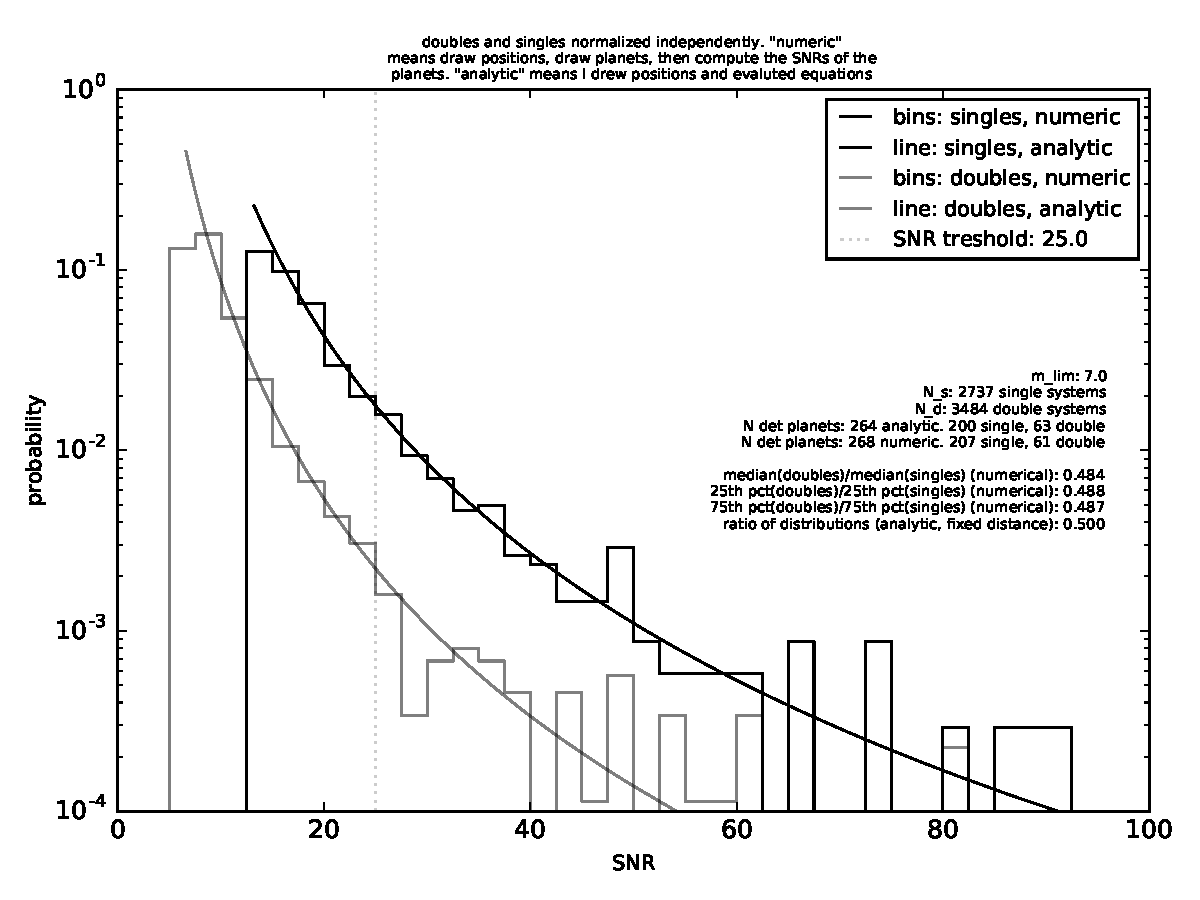
\includegraphics[scale=0.4]{figures/snr_distribution.pdf}
	\end{center}
	\caption{Comparison of analytic and numeric probability 
	density functions of the SNR in an idealized transit survey.
	The analytic lines are Eqs.~\ref{eq:prob_xs} and~\ref{eq:prob_xd} for the 
	planet populations orbiting single and binary stars. The underlying stepped 
	histogram is output from Monte Carlo simulations. Poisson noise leads to 
	a small deviation at the faint and bright limits, but the numerics and 
	analytics otherwise agree.
		 }
	\label{fig:snr_dist_analytic_v_numeric}
\end{figure}


\subsection{Representative numbers for a few cases}

\subsubsection{Twin binaries: if we ignore binarity, for what fraction of 
detections do we misclassify the radii?}
 
Ignoring binarity, we will detect $N_{\rm det,s}$ planets around single stars, 
and $N_{\rm det,d}$ planets around double stars. The latter set will be assumed 
to have radii $R_p \sqrt{\mathcal{D}}$.
The fraction of detections with misclassified radii can then be written
\begin{equation}
\frac{N_{\rm det,d}}{N_{\rm det,s} + N_{\rm det,d}} = \frac{1}{1+\alpha},
\end{equation}
for
\begin{equation}
\alpha \equiv \frac{1}{2({\rm BF})} (1+\gamma_R)^{3/2} 
\frac{\Gamma_{t,s}}{\Gamma_{t,d}}.
\end{equation}

For the nominal G2V dwarf case of ${\rm BF}=0.45$, twin binaries with equal 
occurrence rates this produces a misclassification rate of $24\%$, in agreement 
with Fig.~\ref{fig:snr_dist_analytic_v_numeric}.

\subsubsection{Twin binaries: if we ignore binarity, how wrong is our
occurrence rate for planets of radius $R_p$?}

This is almost simply asking ``what is the relative difference between the 
occurrence rates derived by Astronomers D and A for planets of radius $R_p$?''
However, in the more realistic case, Astronomer A also has derived a 
completeness, which we assume is the same as for Astronomer D in the single 
star case.
So Astronomer A now misclassifies planetary radii, and miscounts the total 
number of stars, but knows his completeness for single stars.
Astronomer D corrects all these errors.
Then
\begin{equation}
\Gamma_{{\rm A}, R_p} = \frac{N_{\rm det,s}/(f_{s,g} f_{s,c})}{N_s + N_d}.
\end{equation}

To express ``how wrong'' our occurrence rate is, we define a correction factor 
$X_\Gamma$ such that the true occurrence rate is the product of the correction 
factor with the measured occurrence rate: $\Gamma_D \equiv \Gamma_A X_\Gamma$.

The correction factor is then
\begin{align}
X_\Gamma &=
\frac{\Gamma_{{\rm D},R_p}}{\Gamma_{{\rm A},R_p}} \\
&=
\frac{\Gamma_{t,s}N_s + 2\Gamma_{t,d}N_d}{N_s + 2N_d}  \cdot 
\frac{N_s + N_d}{\Gamma_{t,s} N_s } \\
&= 
\frac{(1 + \beta)(1 + 2 \beta \Gamma_{t,d}/\Gamma_{t,s})}{(1+2\beta)},
\end{align}
for
\begin{equation}
\beta \equiv N_d/N_s = {\rm BF} \times (1+\gamma_R)^{3/2}.
\end{equation}

For the nominal G2V dwarf case of ${\rm BF}=0.45$ with twin binaries ($\gamma_R 
= 1$) and $\Gamma_{t,d} = \Gamma_{t,s}$ this gives $X_\Gamma = 2.27$.
For instance, in the numerical simulation corresponding to 
Fig.~\ref{fig:snr_dist_analytic_v_numeric}, Astronomer A finds 
$\Gamma_{{\rm A},R_p} = 0.22$, while Astronomer 
D derives the true (input) occurrence rate of $\Gamma_{{\rm D},R_p} = 0.5$.
This gives a relative percentage error of $\delta\Gamma_{{\rm D},R_p} \equiv 
(\Gamma_{\rm A,R_p} - \Gamma_{\rm D,R_p}) / \Gamma_{\rm D,R_p} = -56\%$.



\section{Model \#2: fixed stars, fixed planets, varying light-ratio binaries}
\label{sec:model_2}

Same story as Model \#1, except now $\gamma_R$ varies across the population 
of star systems.
It does so because the underlying mass ratio varies. 
Since we are interested in solar type binaries, we take the distribution of the 
mass ratio $q=M_2/M_1$ by approximating [Rhagavan et al 2010, Fig 16]:
\begin{equation}
{\rm prob}(q) =
\Bigg\{\begin{array}{lr}
c_q & 0.1 < q \leq 1  \\
0 & {\rm otherwise},
\end{array}
\label{eq:mass_ratio}
\end{equation}
for $c_q = 1/9$ to normalize the distribution to 1.
The mass-luminosity relation can, for analytic convenience, be approximated as 
$L = M^\alpha$, with the lore-value of $\alpha$ being $3.5$.
While we use this in subsequent analytic development, for numerics we fit a 
lines to mass-luminosity data collected by Torres et al. [2009] for 
dwarfs above M, and Benedict et al. [2016] for dwarfs below M.
To convert Benedict et al. [2016]'s reported $M_V$ values to absolute 
luminosities, we interpolated over E. Mamajek's 
table\footnote{
	\texttt{pas.rochester.edu/\textasciitilde 
		emamajek/EEM\_dwarf\_UBVIJHK\_colors\_Teff.txt},
	downloaded 2017.08.02}.
In log-log space, we let the intersection point of the lines float, and make 
various cuts on the data as indicated in Fig~\ref{fig:mass_luminosity}. The 
fit parameters are available in a footnote\footnote{
	m lo: 1.8818719873988132~--~
	c lo: -0.9799647314108376~--~
	m hi: 5.1540712426599882~--~
	c hi: 0.0127626185389781~--~
	M at merge: 0.4972991257826812~--~
	L at merge: 0.0281260412126928.
}.
\begin{figure}
	\begin{center}
		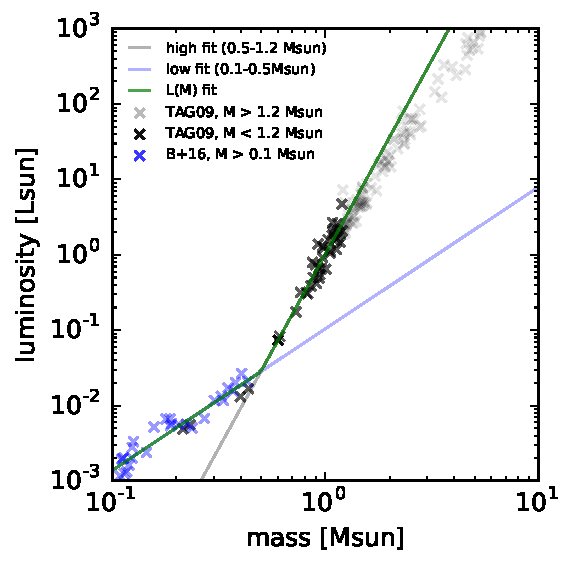
\includegraphics[scale=0.9]{figures/mass_luminosity.pdf}
	\end{center}
	\caption{Empirical fit to main sequence dwarf mass luminosity data compiled 
	from Torres et al. [2009] and Benedict et al. [2016]. The ``low fit'' is a 
	least squares fit to data from $0.1-0.5M_\odot$, and the ``high fit'' is to 
	data above that, and below the Kraft break ($1.2M_\odot$).
	The $L(M)$ relation taken for subsequent numerics is the maximum 
	of the two fits.
	}
	\label{fig:mass_luminosity}
\end{figure}

The other changes between Model \#2 and Model \#1 are:
\begin{enumerate}
\item We allow a third occurrence rate, splitting $\Gamma_{t,d} \rightarrow 
(\Gamma_{t,d1}, \Gamma_{t,d2})$ where the latter terms represent the occurrence 
rate around the primary of a double star system, and the occurrence rate around 
the secondary of a double star system. For the case of \textit{e.g.}, $q=0.1$, 
this seems more relevant.
We can then take the limit that says ``any planet around the secondary is as 
likely as around the primary'', or go to the opposite extreme of ``there are 
only planets around the primaries, not the secondaries''.
%
\item Our binary systems have secondaries with varying masses. Thus they have 
varying radii. Taking [Demircan \& Kahraman 1991]'s empirical fit to eclipsing 
binary data,
\begin{equation}
R = 1.06 M^{0.945}
\label{eq:mass_radius}
\end{equation}
for all the stars in our desired mass range ($M < 1.66M_\odot$, D\&K 1991's 
stated bounds), and for each in solar units. This only affects the transit 
probabilities about the secondaries of binary star systems.
\end{enumerate}

We then ask the same questions as for Model \#1.

\subsection{How many stars are in the sample?}

Let $N_s$ be the number of single star systems, and $N_d$ the number of double 
star systems. $N_s$ is the same as in Sec.~\ref{sec:model_1}.

Now
\begin{equation}
N_d(\gamma_R) = n_d \frac{4\pi}{3} d_{\rm max,d}^3(L_1^N, \gamma_R, F_{\rm 
	lim}^N)
\end{equation}
for
\begin{equation}
d_{\rm max,d}(L_1^N, \gamma_R, F_{\rm lim}^N) =
d_{\rm max,s}(L_1^N, F_{\rm lim}^N)\times (1+\gamma_R)^{1/2}.
\end{equation}
Since $q$ is a random variable, $\gamma_R$ is a random variable, and $d_{\rm 
	max,d}$ is a random variable. Since $N_d$ is a function of $d_{\rm max,d}$, 
the number of double star systems becomes a random variable.
The expected (mean) number of double star systems in the sample is
\begin{equation}
\langle N_d \rangle = \int_{0}^{\infty} N_d\, {\rm prob}(N_d) \,{\rm d}N_d.
\end{equation}
By applying the chain rule for probability density functions, the distribution 
${\rm prob}(N_d)$ can be written 
\begin{equation}
{\rm prob}(N_d) = {\rm prob}(q(\gamma_R)) 
\left| \frac{{\rm d}q}{{\rm d}\gamma_R}  \right|
\left| \frac{{\rm d}\gamma_R}{{\rm d}d_{\rm max,d}}  \right|				
\left| \frac{{\rm d}d_{\rm max,d}}{{\rm d}N_d}  \right|.
\end{equation}
Doing some algebra, and assuming $\gamma_R = q^3$, this can be shown to be
\begin{align}
{\rm prob}(N_d) = \frac{2}{81} &N_d^{-1/3} \left(\frac{3}{4\pi 
	n_d}\right)^{2/3} d_{\rm max,s}^{-2/3} \ \times \nonumber\\
&\left[ \left(\frac{3 N_d}{4\pi n_d}\right)^{2/3} - d_{\rm 
	max,s}^2 \right]^{-2/3}
\end{align}
over the interval
\begin{equation}
{\rm lower\ bound} = \frac{4 \pi n_d}{3} (\sqrt{0.1^3 + 1} d_{\rm max,s})^3
\end{equation}
\begin{equation}
{\rm upper\ bound} = \frac{4 \pi n_d}{3} (\sqrt{2}d_{\rm max,s})^3,
\end{equation}
and outside the stated interval ${\rm prob}(N_d) = 0$.

While a closed analytic expression for $\langle N_d \rangle$ does exist, it is 
messy, and it does not yield much intuition. Instead, summarizing the important 
points and supporting them numerically:
\begin{itemize}
	\item In a volume-limited sample of binary star systems in which the 
	primary mass is fixed, and the mass ratio is drawn from a bounded uniform 
	distribution, the distribution of $\gamma_R$ will be biased towards low 
	values ($\gamma_R \approx 0.1$). This is shown in 
	Fig.~\ref{fig:gammaR_distribn_vol_limited}.
	\item In a magnitude-limited sample of binary star systems in which the 
	primary mass is fixed, and the mass ratio of the \textit{population} is 
	drawn from a bounded uniform distribution, the observed distribution of 
	mass ratios will be biased towards high values. You will see more twins,
	because they are detectable out to a greater distance\footnote{This is a 
	scarcy systematic w.r.t. the claimed intrinsic excess of twin binaries.}. 
	This is shown in 
	Fig.~\ref{fig:q_distribn_mag_limited}.
	\item In a magnitude-limited sample of binary star systems in which the 
	primary mass is fixed, the distribution of $\gamma_R$ will be biased 
	towards low values ($\approx 0.1$), but less so than in a 
	volume-limited sample. This is shown in 
	Fig.~\ref{fig:gammaR_distribn_mag_limited}.
\end{itemize}

In passing, the bias in ${\rm prob}(\gamma_R)$ towards low luminosity ratios 
can be seen analytically. If we assume $\gamma_R = q^\alpha$, then
\begin{equation}
{\rm prob}(\gamma_R) = \frac{1}{9 \alpha} \ \gamma_R^{\frac{1-\alpha}{\alpha}}
\quad {\rm for\ } (0.1)^\alpha < \gamma_R < 1,
\end{equation}
and otherwise zero. For instance if $\alpha = 3$, ${\rm prob}(\gamma_R) 
\propto \gamma_R^{-2/3}$ and the domain extends from $1$ to 
$10^{-3}$, where the probability distribution peaks.

\begin{figure}[!t]
	\begin{center}
		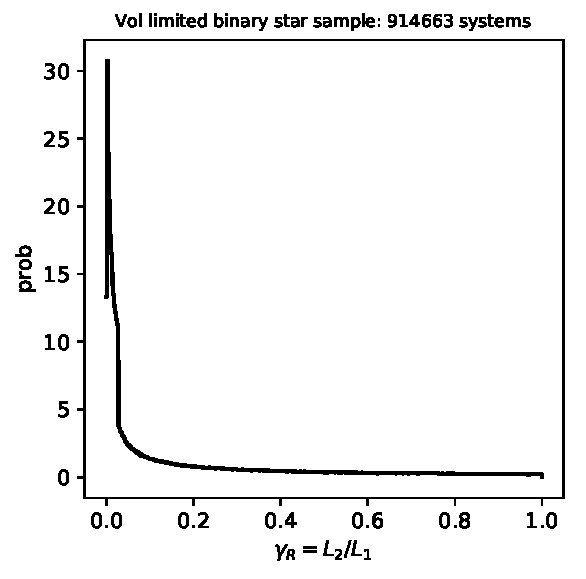
\includegraphics[scale=.8]{figures/gammaR_distribn_vol_limited.pdf}
	\end{center}
	\caption{The distribution of the luminosity ratio for a volume limited 
		sample of binary stars. ${\rm BF} = 0.45$ [Duchene and Kraus 2013]; 
		total 
		number density from Bovy 2017; $M(L)$ relation from 
		Fig.~\ref{fig:mass_luminosity}; mass ratios are drawn from 
		Eq.~\ref{eq:mass_ratio}.}
	\label{fig:gammaR_distribn_vol_limited}
\end{figure}
\begin{figure}[!t]
	\begin{center}
		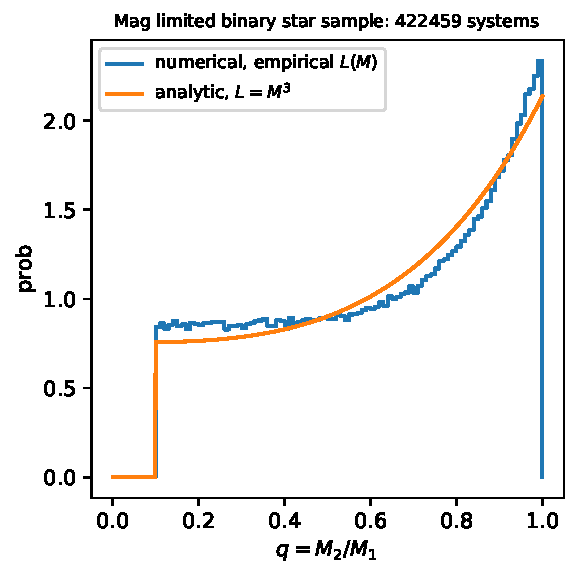
\includegraphics[scale=.8]{figures/q_distribn_mag_limited.pdf}
	\end{center}
	\caption{The distribution of the mass ratio for a magnitude limited 
		sample of binary stars. ${\rm BF} = 0.45$ [Duchene and Kraus 2013]; 
		total 
		number density from Bovy 2017; $M(L)$ relation from 
		Fig.~\ref{fig:mass_luminosity}; mass ratios are drawn from 
		Eq.~\ref{eq:mass_ratio} -- a \textit{uniform} distribution in a 
		volume-limited sample!}
	\label{fig:q_distribn_mag_limited}
\end{figure}
\begin{figure}[!t]
	\begin{center}
		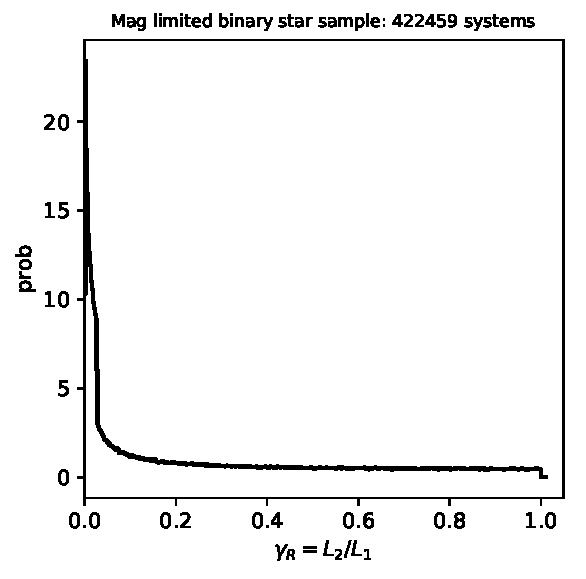
\includegraphics[scale=.8]{figures/gammaR_distribn_mag_limited.pdf}
	\end{center}
	\caption{The distribution of the luminosity ratio for a magnitude limited 
		sample of binary stars. ${\rm BF} = 0.45$ [Duchene and Kraus 2013]; 
		total 
		number density from Bovy 2017; $M(L)$ relation from 
		Fig.~\ref{fig:mass_luminosity}; mass ratios are drawn from 
		Eq.~\ref{eq:mass_ratio}.}
	\label{fig:gammaR_distribn_mag_limited}
\end{figure}

\paragraph{How many stars are in the sample?}

We return to the original question: how many stars?
\begin{equation}
\langle N_{\rm stars} \rangle = N_s + 2 \langle N_d \rangle,
\end{equation}
as before.
Since we are not giving analytic expressions for either of the $\langle \ldots 
\rangle$ terms, we just note that in the case of a population with a single 
$\gamma_R$ value, $N_d/N_s = {\rm BF} \times (1 + \gamma_R)^{3/2}$. A lower
bound for this ratio will always be the binary fraction.
For a single run of a Monte Carlo code, where ${\rm mean}(\gamma_R) = 0.28$, 
${\rm median}(\gamma_R) = 0.13$, and the distribution was that given in 
Fig.~\ref{fig:gammaR_distribn_mag_limited}, the observed ratio was $N_d/N_s = 
0.59$.
This corresponds to a single-valued population with $\gamma_R \sim 0.20$, a
number between the mean and median of the true distribution.
It means $\sim 1.2$ stars in binary star systems for every star in a single 
star system from this sample.

We also note in passing that $N_d/N_s = 0.59$ is a smaller ratio than for the 
case of a fixed $\gamma_R$ population with $\gamma_R = 1$, which gave $N_d/N_s 
= 1.27$. The difference is that in the latter population, the volume of 
searchable stars is greater. Based on the fixed-$\gamma_R$ population scaling 
law $N_d / N_s \propto (1+\gamma_R)^{3/2}$, we 
would expect the ratio of single stars to be $\sim (2/1.1)^{3/2} = 2.4$ 
times smaller, which is roughly (though not exactly) what we observe.



\subsection{How many planets are in the sample?}

The mean number of planets in the sample is
\begin{align}
\langle N_{\rm planets} \rangle
=& N_{\rm planets\ in\ single\ star\ systems}  +  \\
&\quad\quad N_{\rm planets\ in\ double\ star\ systems} 
\nonumber \\
=& \Gamma_{t,s} N_s + (\Gamma_{t,d1} + \Gamma_{t,d2}) \langle N_d \rangle.
\end{align}

What was formerly a factor of 2 has now been split into the true occurrence 
rates about the primaries and secondaries of double star systems.

\subsection{What is the true occurrence rate?}

The ``true occurrence rate'' is the average number of planets per star. Thus

\begin{align}
\Gamma_t &= \frac{\langle N_{\rm planets}\rangle}{\langle N_{\rm stars} 
\rangle} \\
\Gamma_t &= \frac{\Gamma_{t,s} N_s + (\Gamma_{t,d1} + \Gamma_{t,d2}) \langle 
N_d\rangle}{N_s +	2\langle N_d\rangle}.
\label{eq:true_occ_2}
\end{align}



\subsection{How many planets are detected?}

The total number of planet detections is the sum of the number of planets 
detected in single star systems $N_{{\rm det},s}$ and the number of planets 
detected in double star systems $N_{{\rm det},d}$.
The latter of these is a random variable, and can be further split into the 
primary and secondary contributions $N_{{\rm det},d1}$, $N_{{\rm det},d2}$.

The number of planets detected in single star systems is
\begin{equation}
N_{{\rm det},s} = N_s \Gamma_{t,s} f_{s,g} f_{s,c},
\end{equation}
where the product $N_s \Gamma_{t,s}$ is the number of planets in the single 
star systems of the sample, $f_{s,g}$ is the geometric probability of the 
planets transiting, and $f_{s,c}$ is the fraction of transiting planets around 
single star systems that are detected (the completeness).


The mean number of planets detected in double star systems is
\begin{equation}
\langle N_{{\rm det},d}\rangle = \langle N_d\rangle  
(\Gamma_{t,d1} f_{d1,g} f_{d1,c} + 
\Gamma_{t,d2} f_{d2,g} f_{d2,c} ).
\label{eq:N_det_d_2}
\end{equation}
Now $\langle N_d\rangle  \Gamma_{t,d1}$ is the mean number of planets orbiting 
the primaries of double star systems, ditto the corresponding expression for 
the secondaries.
For this population, $f_{d1,g} = f_{s,g}$, but $f_{d1,g} \neq f_{d2,g}$.
The completeness fractions differ between the primary and secondary because 
the dilution as a function of the light ratio, $\mathcal{D}(\gamma_R)$, has 
different behavior for the two cases.
We show this in Fig.~\ref{fig:rad_vs_gammaR}.
Specifically, a planet orbiting the secondary will have worse dilution than a 
planet orbiting the primary, and consequently lower completeness.

\begin{figure}[!t]
	\begin{center}
		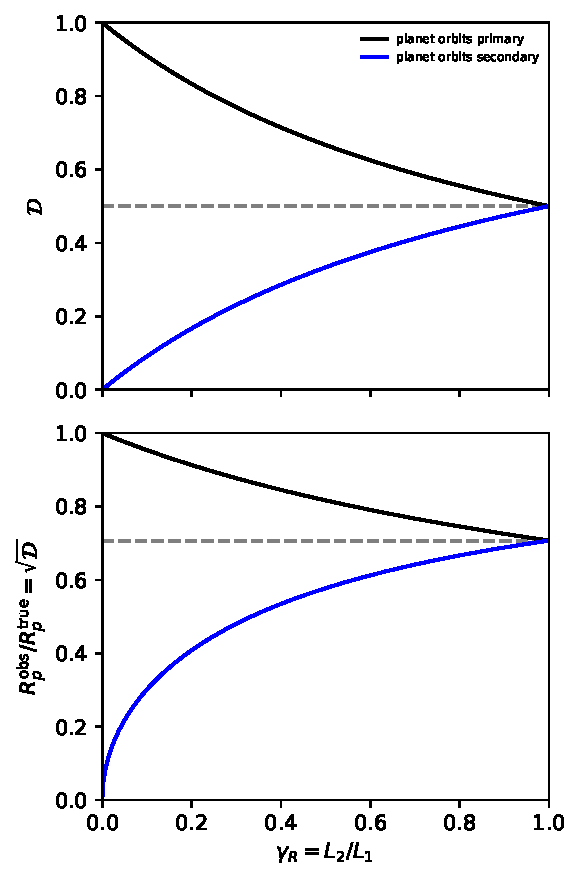
\includegraphics[scale=.9]{figures/observed_radii_vs_gammaR.pdf}
	\end{center}
	\caption{Dilution $\mathcal{D}$ and observed to true radius ratio 
	$\sqrt{\mathcal{D}}$ plotted against binary light ratio $\gamma_R$. This 
	illustrates	Eq.~\ref{eq:dilution}. The lower panel's horizontal line is at 
	$1/\sqrt{2}$.
	The implication is that if a detected planet orbits the secondary and you do 
	not know it, you cannot measure $R_p$ to better than $\approx 29\%$ 
	accuracy.
	Conversely, if it orbits the primary and you do not know it, you will get 
	the radius wrong by at most $\approx 29\%$.
	}
	\label{fig:rad_vs_gammaR}
\end{figure}

We could probably derive analytic expressions for all the terms between 
brackets in Eq.~\ref{eq:N_det_d_2}, completeness included.
I'm not yet convinced we need to -- we should get cancellations for
most of the questions we want to ask.

\subsubsection{Analytic completeness}
\texttt{todo, if necessary}
\subsubsection{Deriving ${\rm prob}(x_i)$}
\texttt{todo, if necessary}
\subsubsection{Number of detected planets}
\texttt{todo, if necessary}

\subsection{Astronomer A ignores binarity}

Just as in Sec.~\ref{sec:model_1}, Astronomer A
\begin{itemize}
\item has never heard about binary star systems.
\item has never heard about completeness corrections.
\item knows about geometric transit probabilities.
\end{itemize}

What occurrence rate does he derive for planets of radius $R_p$ and period $P$?

The answer is the same as in Sec.~\ref{sec:model_1},
\begin{equation}
\Gamma_{{\rm A}, R_p} = \frac{N_{\rm det,s}/f_{s,g}}{N_s + N_d}.
\end{equation}

However, now rather than planets detected in binary systems being perceived as 
a second population of planets with fixed radius $R_p \sqrt{\mathcal{D}}$, 
there will be an apparent spectrum of diluted radii, since $\mathcal{D}$ 
varies by system.
Writing the number of detections in double systems as a function of observed 
radius, $N_{\rm det,d}(R_p^{\rm obs})$, Astronomer A would derive an 
occurrence rate for this separate population of
\begin{equation}
\Gamma_{\rm A}(R_p^{\rm obs}) = \frac{N_{\rm det,d}(R_p^{\rm 
obs})/f_{s,g}}{N_s + N_d}.
\end{equation}
Note that this astronomer thinks these planets orbit single stars, 
and so miscomputes the geometric transit probability for the secondaries.

A more realistic question is ``what fraction of multiples have $\gamma_R$ 
smaller enough so that you'd still observe a radius close to the true one?''. 
We discuss this in Sec.~\ref{sec:close_enough}.

\subsection{Astronomer B counts host stars correctly}

Same as astronomer A above, except the denominator becomes $N_s + 2N_d$.

\subsection{Astronomer C counts host stars correctly and figures out diluted
radii}

In Sec.~\ref{sec:model_1}, Astronomer C only had to do high resolution 
imaging to measure $\gamma_R$ for each system. Since for $\gamma_R = 1$, the 
dilution is single-valued (Fig.~\ref{fig:rad_vs_gammaR}), this immediately 
told her the true planet radius (since the primary/secondary distinction was 
meaningless).

In Model \#2's universe, the dilution is double-valued for a given $\gamma_R$.
To correctly work out the diluted radii, Astronomer C now needs more than high 
resolution imaging -- she needs to resolve the stars during transit to 
discover which star the planet orbits.
She also needs to derive masses for the primaries and secondaries (to make the 
geometric transit probability correction).

Only after doing this does she find that all detected planets from this survey 
have radii $R_p$. She computes an occurrence rate
\begin{equation}
	\Gamma_{{\rm C},R_p} = 
	\frac
			{N_{\rm det,s}/f_{s,g} +
			  N_{\rm det,d1}/f_{d1,g} +
			  N_{\rm 	det,d2}/f_{d2,g}}
			{N_s + 2N_d}
\end{equation}

the closest yet to the true rate (Sec.~\ref{sec:true_rate}).


\subsection{Astronomer D counts host stars correctly, figures out diluted
radii, and accounts for completeness}

Same story as for Model \#1.
Now, they do injection recovery and derive correct estimates for their 
completeness functions about single stars $f_{s,c}$, the primaries of double 
star systems, $f_{d1,c}$, and the secondaries of double star systems 
$f_{d2,c}$.
They compute the respective single and binary 
occurrence rates
\begin{equation}
\Gamma_{t,s} = \frac{N_{\rm det,s}}{N_s f_{s,g} f_{s,c}},
\end{equation}
\begin{equation}
\Gamma_{t,d1} = \frac{N_{\rm det,d1}}{N_d f_{d1,g} f_{d1,c}},
\end{equation}
\begin{equation}
\Gamma_{t,d2} = \frac{N_{\rm det,d2}}{N_d f_{d2,g} f_{d2,c}}.
\end{equation}

With these in hand, they derive the overall occurrence rate
\begin{align}
\Gamma_{{\rm D}, R_p} 
&= \frac{
	N_{\rm det,s}/f_s + 
	N_{\rm det,d1}/f_{d1} +
	N_{\rm det,d2}/f_{d2}
	}
	{N_s + 2 N_d} \\
&= \frac{\Gamma_{t,s} N_s + (\Gamma_{t,d1} + \Gamma_{t,d2})N_d}
				{N_s + 2 N_d},
\end{align}
where $f_s \equiv f_{s,g}f_{s,c}, f_{d1} \equiv f_{d1,g}f_{d1,c}, 
f_{d2} \equiv f_{d2,g}f_{d2,c}$ for brevity.
Astronomer D's occurrence rate is the true occurrence rate (cf. 
Eq.~\ref{eq:true_occ_2}).


\subsection{Numerical verification}
\texttt{todo, if needed}


\subsection{Representative numbers for a few cases}

We have not given analytic expressions for the number of double star systems 
$N_d$ because even with simplified $M(L)$ relations, they are unwieldy.
However, we can ask similar numerical questions as from Sec.~\ref{sec:model_1}, 
and compare the answers.


\subsubsection{If we ignore binarity, for what fraction of detections do we
misclassify the radii?}

Ignoring binarity, we will detect $N_{\rm det,s}$ planets around single stars, 
and $N_{\rm det,d}$ planets around double stars. The latter set will be assumed 
to have radii $R_p \sqrt{\mathcal{D}}$, where $\mathcal{D}$ is the vector of 
dilutions appropriate for each binary star system.
The fraction of detections with misclassified radii can then be written
\begin{equation}
\frac{N_{\rm det,d}}{N_{\rm det,s} + N_{\rm det,d}} = \frac{1}{1+\alpha},
\end{equation}
for
\begin{equation}
\alpha \equiv 
\frac{ N_d (\Gamma_{t,d1} f_{d1} + \Gamma_{t,d2} f_{d2}) }{N_s \Gamma_{t,s} 
f_s},
\end{equation}
where $f_s \equiv f_{s,g}f_{s,c}, f_{d1} \equiv f_{d1,g}f_{d1,c}, 
f_{d2} \equiv f_{d2,g}f_{d2,c}$ for brevity.

% For the nominal G2V dwarf case of ${\rm BF}=0.45$, and the same distributions 
% used to generate 
% Figs.~\ref{fig:gammaR_distribn_vol_limited}~--~\ref{fig:gammaR_distribn_mag_limited},
% we found $N_d/N_s=0.59$.
% We are assuming $\Gamma_{t,d} / \Gamma_{t,s} = 1$.
% If we maintained the (incorrect) assumption that $f_{d,{\rm geom}} / f_{s,{\rm 
% 		geom}} = 1$, this would give a misclassification rate of 45\%. 
% 
% This latter assumption is wrong because although we are letting the occurrence 
% rate be the same across binary and single systems, our binary systems have 
% secondaries with varying masses. Thus they have varying radii.
% Taking [Demircan \& Kahraman 1991]'s empirical fit to eclipsing binary data,
% \begin{equation}
% R = 1.06 M^{0.945}
% \label{eq:mass_radius}
% \end{equation}
% for all the stars in our desired mass range ($M < 1.66M_\odot$, D\&K 1991's 
% stated bounds).
% For a zero eccentricity system, $f_{\rm geom}=R_\star/a$.
% Since $f_{d,{\rm geom}} = 0.5\times (f_{d1,{\rm geom}} + f_{d2,{\rm geom}})$, 
% \textit{i.e.} it is the average of the transit probabilities for both the 
% primary and secondary (d1 and d2), we can write (dropping the ``geom'' 
% subscript)
% \begin{align}
% \frac{f_d}{f_s} &= \frac{1}{2} \left(1 + \left(\frac{M_1}{M_{d2}}\right)^{1/3} 
% \frac{R_{d2}}{R_1}\right) \\
% &= \frac{1}{2} \left( 1 + q^{-1/3 + 0.945}\right).
% \end{align}
% 
% Computing it all out in a numerical simulation, the only thing that changes 
% analytically is that
% \begin{equation}
% N_d f_d \rightarrow \sum_{i=1}^{N_d} f_{d,i},
% \end{equation}
% so when considering the ratio $f_d/f_s$, we are in fact interested in
% \begin{equation}
% \frac{\langle f_d \rangle}{f_s} = \frac{\frac{1}{N_d} \sum_{i=1}^{N_d} 
% 	f_{d,i}}{f_s},
% \end{equation}
% where $f_{d,i}$ is the vector of geometric transit probabilities across all 
% systems.
% For the same numerical realization with $N_d/N_s = 0.59$, and using the mass 
% radius relation given by Eq.~\ref{eq:mass_radius}, I get $\langle f_d 
% \rangle / f_s = 0.84$ (smaller secondaries lead to a smaller average transit 
% probability in double star systems), for a radius misclassification rate of 
% $0.51$.


\texttt{The different secondary completeness matters here if proceeding 
analytically. Would be easier to do numerically.
Regardless, this is not the most interesting question right now.}

\subsubsection{If we ignore binarity, how wrong is our occurrence rate for
planets of radius $R_p$?}
\label{subsubsec:model2_A}

Write $\Gamma_{{\rm A,\ planets\ of\ }R_p} = \Gamma_{{\rm A,}R_p}$, 
and similarly for ${\rm D}$.
Just as in Model \#1, the answer to ``what is the relative difference between 
the occurrence rates derived by Astronomers D and A for planets of radius 
$R_p$?''
is simpler when we assume that Astronomer A has also derived a 
completeness, which we assume is the same as for Astronomer D in the single 
star case.
So Astronomer A now misclassifies planetary radii, and miscounts the total 
number of stars, but somehow knows his completeness for single 
stars. This is possible, because Astronomer A can correctly derive a 
completeness estimate and geometric transit probability for single stars only. 
For Astronomer $A'$ below, including the planets in binary star systems in the 
numerator introduces mistakes in the estimated completeness, and so the picture 
is more complicated.
Then
\begin{equation}
	\Gamma_{{\rm A}, R_p} = \frac{N_{\rm det,s}/(f_{s,g} f_{s,c})}{N_s + N_d}.
\end{equation}

The correction factor $X_\Gamma$ is
\begin{align}
X_\Gamma &=
\frac{\Gamma_{{\rm D},R_p}}{\Gamma_{{\rm A},R_p}} \\
&=
\frac{\Gamma_{t,s}N_s + (\Gamma_{t,d1} + 
	\Gamma_{t,d2})N_d}{N_s + 2N_d}  
\cdot 
\frac{N_s + N_d}{\Gamma_{t,s} N_s } \\
&= 
\frac{(1 + \beta (\Gamma_{t,d1}+\Gamma_{t,d2})/\Gamma_{t,s})(1 + 
	\beta)}{(1+2\beta)} 	\\
&=
(1 + \chi \beta )
\cdot 
\frac{1 + \beta}{1 + 2\beta }
\end{align} 
for
\begin{equation}
\beta \equiv N_d/N_s, \quad \chi \equiv 
(\Gamma_{t,d1}+\Gamma_{t,d2})/\Gamma_{t,s}.
\end{equation}

In the limit where the $R_p$ planet has the same occurrence rate about every 
host type regardless of its mass, $\chi=2$, and this simplifies to $X_\Gamma = 
1+\beta$.
This is same expression as what we found for Model \#1, but now the value of 
$\beta$ will be smaller in this model because of the 
smaller volume of searchable binary stars.
From numerics, we find $\beta = N_d/N_s = 0.59$, so the occurrence rate 
correction factor is $X_\Gamma(\chi=2) = 1.59$.

If we consider the opposite limit of the $R_p$ planet \textit{only} 
existing around single stars and the primaries of double star systems with 
equal occurrence, $\chi = 1$, and $X_\Gamma = (1 +\beta)^2 / (1+2\beta)$.
For $\beta = 0.59$, this gives $X_\Gamma(\chi=1) = 1.16$.
The true correction factor is somewhere between these two limits.



\subsubsection{What if we ignore binarity, but count derived planet radii that 
are ``close enough''?}
\label{sec:close_enough}

Let $x$ be the acceptable margin of error on the observed radius, so that we 
are interested in counting the number of planets detected with $R_p < R_p^{\rm 
obs} < (1\pm x) R_p$.
For Model \#2, since all planets have radius $R_p$, we only care about 
the smaller radius case, \textit{i.e.}, we want to count $R_p > R_p^{\rm 
	obs} > (1 - x) R_p$, for instance with $x=0.1$.

The diluted detections only occur in binary systems. The number of 
planets detected in double star systems with observed radius $R_p^{\rm obs}$ 
is
\begin{align}
N_{\rm det,d}(R_p^{\rm obs}) &= N_{\rm det, d1}(R_p^{\rm obs}) + 
								N_{\rm det, d2}(R_p^{\rm obs}) \\
&= \Gamma_{t,d1} f_{d1}(R_p^{\rm obs}) N_{d1}(R_p^{\rm obs})\  + \nonumber \\
&\quad\quad \quad\Gamma_{t,d2} f_{d2}(R_p^{\rm obs}) N_{d2}(R_p^{\rm obs}).
\end{align}
As always, the fractional terms $f_{di}$ for $i\in{1,2}$ encompass geometric 
and completeness corrections.
We're writing both them and the number of stars for which a given observed 
radius would be seen as functions of $R_p^{\rm obs}$.

To save on notational horribleness, write $R_p' \equiv \{(1-x) R_p < R_p^{\rm 
obs} < R_p\}$, in other words let $R_p'$ denote the set of planets that are 
observed in the desired radius range.

Then writing $N_{d1}(R_p')$, the number of double systems for which a $(R_p, 
P)$ planet would be observed in $R_p'$ if it orbiting the primary, is 
relatively straight-forward:
\begin{equation}
N_{d1}(R_p') = \int_{0}^{{\rm min}(1,\gamma_{R,u})} N_d(\gamma_R) 
\,{\rm prob}(\gamma_R) \,{\rm d}(\gamma_R),
\label{eq:N_d1}
\end{equation}
where the upper limit is set by equating the limiting radius $(1-x)R_p$ to the 
observed diluted radius $(1+\gamma_R)^{-1/2}R_p$, giving
\begin{equation}
\gamma_{R,u} \equiv \frac{x (2-x)}{(1-x)^2}.
\end{equation}
If $x > (1 - 2^{-1/2})$, bad things happen (cf. Fig.~\ref{fig:rad_vs_gammaR}), 
hence the need for the minimum.
Note that Eq.~\ref{eq:N_d1} is not an expression for the number of detected 
planets about primaries -- that quantity is expressed as $\Gamma_{t,d1} 
f_{d1}(R_p^{\rm obs}) N_{d1}(R_p^{\rm obs})$.

The analogous equation to Eq.~\ref{eq:N_d1} for $N_{d2}(R_p')$, the number of 
double systems for which a $(R_p, P)$ planet would be observed in $R_p'$ if it 
orbited the secondary, is
\begin{equation}
N_{d2}(R_p') = 
  \Bigg\{\begin{array}{lr}
  \int_{\gamma_{R,l}}^{1} N_d(\gamma_R)
  \,{\rm prob}(\gamma_R) \,{\rm d}(\gamma_R),\\ 
  \quad\quad\quad\quad\quad\quad\quad\quad x > 1 - 
  2^{-1/2}\\
  0, \quad\quad\quad\quad\quad\quad\quad x \leq 1 - 2^{-1/2} % lol
  \end{array}
\label{eq:N_Rp_secondary}
\end{equation}
where
\begin{equation}
\gamma_{R,l} \equiv \frac{(1-x)^2}{x (2-x)}.
\end{equation}
Eq.~\ref{eq:N_Rp_secondary} accounts for the fact that you cannot measure 
$R_p$ to better than $\approx 29\%$ if the planet orbits the secondary of an 
unidentified binary.
This was originally noted in Fig.~\ref{fig:rad_vs_gammaR}.

If we were forward-modelling, \textit{i.e.} if we actually wanted to compute 
$N_{\rm det,d}(R_p')$, we would also need to evaluate the total detection 
efficiency term $f_{d1}(R_p^{\rm obs})$, which is a product of the geometric 
transit probability and the fraction of signals of a given depth that are 
detectable.
We would need to integrate this product over the domain of allowable radii 
$R_p'$ to find the number of detected planets.

However, the procedure of estimating the geometric transit probability, as well 
as the completeness, is complicated by the errors that are introduced by 
including binary star systems that are thought to be single in the numerator.
These stars will have incorrectly estimated masses and radii, which influences 
both $f_c(R_p')$ and $f_g(R_p')$.

\texttt{If we ask the right question, we will not need to actually compute 
either term.}

Astronomer A misclassifies planetary radii, miscounts the total number of 
stars, and (incorrectly) estimates his completeness and geometric correction 
for ``single'' stars as a function of radius $f(R_p')$ (omitting a ``s'' 
subscript because the stars for which this incorrect occurrence rate are 
derived are not all single).
His occurrence rate for planets of radius \textit{near} $R_p$, \textit{i.e.} 
the set of planets with $\{ (1-x)R_p < R_p^{\rm obs} < R_p \}$, is
\begin{equation}
\Gamma_{{\rm A}, R_p'} = \frac{ (N_{\rm det,s} + N_{\rm det,d}(R_p')) 
/ f(R_p')   }{ N_s + N_d}.
\end{equation}

For him,
\begin{equation}
f(R_p') = f_g(R_p') f_c(R_p').
\end{equation}

Astronomer D, who had everything right, changes nothing.

The new correction factor is
\begin{align}
X_\Gamma &= \frac{\Gamma_{{\rm D},R_p}}{\Gamma_{{\rm A},R_p'} } \\
&=
\frac{1+\chi \beta}{1 + \xi}  \cdot 
\frac{1 + \beta}{1 + 2\beta},
\end{align}
for
\begin{equation}
\beta \equiv N_d/N_s, \quad \chi \equiv (\Gamma_{t,d1} + 
\Gamma_{t,d2})/\Gamma_{t,s},
\end{equation}
and
\begin{equation}
\xi \equiv \frac{N_{\rm det,d}(R_p')}{f(R_p')} \cdot \frac{1}{N_s 
\Gamma_{t,s}}.
\end{equation}
If we let $x < 1 - 2^{-1/2}$, for instance $x=0.1$, then $N_{d2}(R_p') = 0$. 
The expression for $\xi$ in this case becomes
\begin{align}
\xi &= \frac{N_{d1}(R_p')}{N_s} \cdot \frac{\Gamma_{t,d1}}{\Gamma_{t,s}} \cdot 
\frac{f_{d1}(R_p')}{f(R_p')} \\
&= \frac{N_{d1}(R_p')}{N_s} \cdot \frac{\Gamma_{t,d1}}{\Gamma_{t,s}} \cdot 
\frac{f_{g,d1}(R_p')}{f_g(R_p')}\cdot \frac{f_{c,d1}(R_p')}{f_c(R_p')},
\label{eq:chi_simplified}
\end{align}
provided that $x < 1-2^{-1/2}$.

We have now parametrized our ignorance.
The values that the latter two ratios of Eq.~\ref{eq:chi_simplified} take 
depend on what we assume Astronomer A' does to derive the stellar parameters 
for the systems that he thinks are singles but are in fact doubles.
For instance, assume he somehow observed the bolometric flux from every point 
on the sky, and used it with a distance to obtain single-star luminosities, and 
thus radii and masses.
His binary systems (thought to be singles) would be bluer than either component 
star is in reality.
On the main sequence, $\rho_\star$ decreases with increasing stellar radius, 
so $\rho_\star$ would be underestimated for all binaries.
Since $f_g \propto \rho_\star^{1/3}$, this means that $f_{g,d1}(R_p')/f_g(R_p') 
> 1$.
However, by the same token we can place an \textit{upper} bound on this ratio. 
In the worst case scenario a given star's luminosity is twice the individual 
star's luminosity. If $L\propto M^3 \propto R^3$, then the radius is 
over-estimated by at most a factor of $2^{1/3}$. Thus the density is 
underestimated by at most a factor of $2^{1/2}$, and $f_g(R_p')$ is 
underestimated by at most a factor of $2^{1/6}=1.12$. 

This begins to take us somewhere. The left-most term of 
Eq.~\ref{eq:chi_simplified} is bounded above by $\beta$. This is because 
$N_{d1}(R_p') \leq N_{d1} = N_d$.
If we assume $\Gamma_{t,d1} = \Gamma_{t,s}$, as we were doing 
anyway, then the product of the three left-most fractions must be less than 
$1.12\beta$.
The only thing standing in our way of an analytic upper bound to $\xi$ is the 
completeness fraction $f_{c,d1}(R_p')/f_c(R_p')$.
Note that over a fixed radius interval dilution will always 
yield a lower completeness fraction for double star systems than singles, so 
$f_{c,d1}(R_p') / f_{c,s}(R_p') \leq 1$.

For the completeness term, an argument that I don't wholly believe
is that
\begin{equation}
\frac{f_{c,d1}(R_p')}{f_c(R_p')} = \frac{f_{c,d1}(R_p')}{f_{c,s}(R_p')} \cdot
	\frac{f_{c,s}(R_p')}{f_{c}(R_p')} \lessapprox 1 \cdot (1+\langle \gamma_R 
	\rangle)^3,
\end{equation}
where the first part of the inequality is obvious, but the second is by 
assuming it's $\lessapprox f_{s,c}/f_{d,c}$, which might be wrong because of 
the radius dependence.

A way of making the estimate without deriving the actual 
completeness fractions, or even running numerics, is just to plot the error as 
a function of $\xi$. We do this in Fig.~\ref{fig:XGamma_vs_xi}, which 
shows that the correction factor varies from 0.6 to 1.6, depending on what 
fraction of secondaries you assume host planets.
\todo[inline]{I could run numerics for this to make the result more 
interesting.}

\begin{figure}[!t]
	\begin{center}
		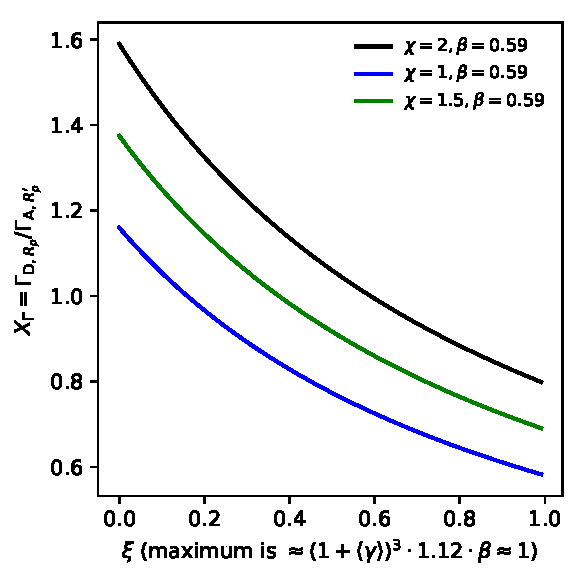
\includegraphics[scale=.8]{figures/XGamma_vs_xi.pdf}
	\end{center}
	\caption{\textit{Y axis}: correction factor for the astronomer who 
	ignores binarity but counts planetary radii that are ``close enough'' (A') 
	and the astronomer who knows everything (D).
	\textit{X axis}: $\chi$ as defined in Eq.~\ref{eq:chi_simplified}. Taking a 
	guess at the true value, if $N_{d1}(R_p') = N_d/2$, and the occurrence rates 
	between `d1' and `s' are the same, and we put $\gamma_R = 0.1$ into the 
	completeness ratio, then $\xi = (\beta/2) \times (1+0.1)^{-3} = 0.22$. The 
	relative error then varies between $\approx 5\% - 35\%$, depending on what 
	fraction of secondaries you assume host planets.
		}
	\label{fig:XGamma_vs_xi}
\end{figure}



\section{Model \# 3: A Synthetic {\it Kepler} Analog}

If we assume every KIC star to be single, what order of magnitude of error do 
we make in occurrence rates estimated for planets of different sizes (and 
periods)?

We can attempt an answer with Monte Carlo simulations of something like the 
\kepler\ field. I say ``something like'' because the binarity properties of the 
\kepler\ field (or more specifically the stars selected in the KIC) are not 
known.
\todo[inline]{but it might be better to do something directly on the KIC's 
selected target stars, like what Ciardi did! The following is a good example, 
but at most it can ``suggest'' that a similar level of error has been made from 
the \kepler\ survey.}

The plan is as follows:
\begin{itemize}
	\item Verify Galaxia can produce something resembling the KIC.
	\item Introduce binaries (Galaxia does not, by default, have any).
	\item Use Galaxia [Sharma et al 2010] to construct an analog of the KIC.
	\item Introduce a planet population.
	\item Numerically assess what occurrence rates would be derived, and 
	compare to previous sections.
\end{itemize}

\subsection{Verifying Galaxia can produce a KIC analog }

Galaxia [Sharma et al 2010] is a stellar population synthesis code for creating 
surveys of the Milky Way. It samples an assumed analytic distribution function. 
In other words, it assumes a number density of stars as a function of position, 
velocity, age, metallicty, and mass, from which it then samples to construct a 
``realistic'' stellar population.
The assumed model includes:
\begin{itemize}
	\item A metallicity distribution (log-normal),
	\item A velocity distribution (triaxial Gaussian),
	\item The stellar density and galactic components specified by Robin et al 
	[2003] (the Besan\c{c}on model) -- see Sharma et al [2010] Table 1. This 
	includes the IMF for a young and old thin disk, a thick disk, a spheroidal 
	component, a bulge component, as well as an ISM and dark halo. It also 
	includes the star-formation rate.
\end{itemize}

While this model of course lacks some detail, Sharma et al [2010] show that 
agreement with the volume-limited Hipparcos sample is probably good enough for 
our purpose of estimating the number of ``solar-like'' (by definition 
hereafter, $0.7 M_\odot < M_\star < 1.3 M_\odot$) stars in something like the 
\kepler\ field.

We then run the Galaxia in its ``circular survey'' mode, towards the direction 
of the \kepler\ field\footnote{galactic longitude 76.532562, galactic latitude 
13.289502.}. We apply the Schlegel, Finkbeiner et al [1999] extinction map when 
converting absolute to apparent magnitudes.

To verify the results are in reasonable agreement with the stars that actually 
exist in that direction, we compare the output with the KIC\footnote{From 
\url{http://archive.stsci.edu/kepler/kic.html}, we 
downloaded the 13.1 million row "|"-delimited gzipped ASCII file containing the 
complete Kepler Input Catalog (version 10).} [Brown et al 2011].
Following Sharma et al [2016, ApJ 822:15], for each catalog we selected all 
stars within $7.5^\circ$ of the center of the \kepler\ field, and with Sloan $r 
< 14$.
The KIC is complete to magnitudes fainter than $r=14$, so the comparison should 
not be affected by its completeness.

\begin{figure}[!t]
	\begin{center}
		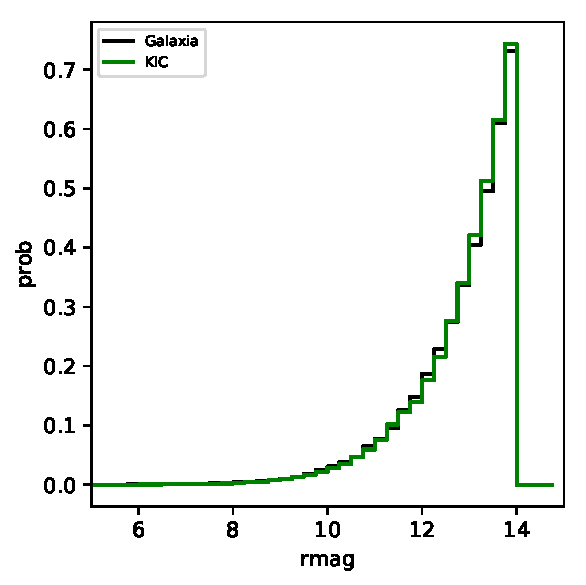
\includegraphics[scale=.8]{figures/rmag_distribn.pdf}
	\end{center}
	\caption{Probably density distributions of $r$ magnitude for $r<14$ stars 
	within $7.5^\circ$ of the center of the \kepler\ field, for Galaxia and the 
	KIC.	}
	\label{fig:rmag_distribn}
\end{figure}
\begin{figure}[!t]
	\begin{center}
		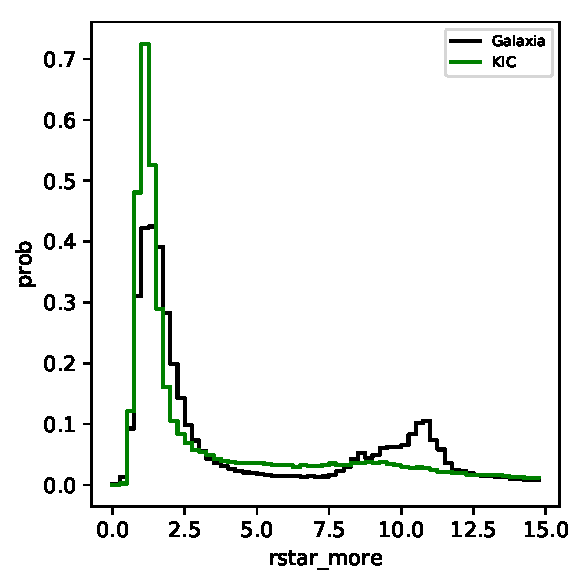
\includegraphics[scale=.8]{figures/rstar_more_distribn.pdf}
	\end{center}
	\caption{Same as Fig.~\ref{fig:rmag_distribn}, for $R_\star$.}
	\label{fig:rstar_more_distribn}
\end{figure}
\begin{figure}[!t]
	\begin{center}
		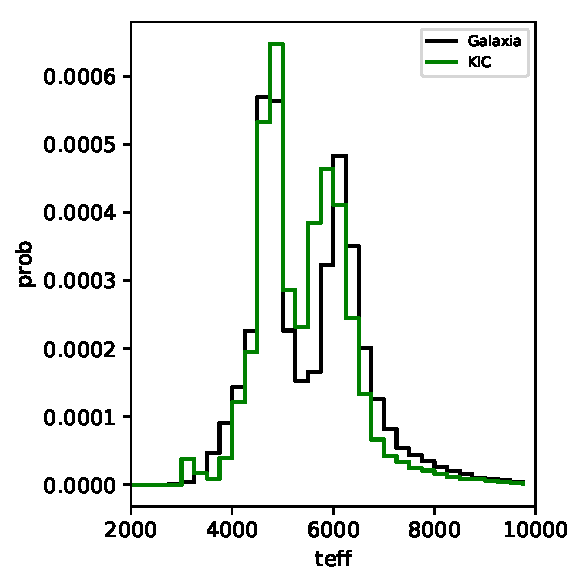
\includegraphics[scale=.8]{figures/teff_distribn.pdf}
	\end{center}
	\caption{Same as Fig.~\ref{fig:rmag_distribn}, for $T_{\rm eff}$.}
	\label{fig:teff_distribn}
\end{figure}

A few distributions are shown in 
Figs.~\ref{fig:rmag_distribn}-~\ref{fig:teff_distribn}.
From Fig.~\ref{fig:rmag_distribn}, we can see that the stellar counts as a 
function of Sloan $r$ magnitude are in close agreement with the KIC.
From Fig.~\ref{fig:rstar_more_distribn}, the KIC reports relatively more dwarf 
stars, and fewer giants than Galaxia does.
This is likely related to KIC's inability to distinguish between dwarfs and 
giants with only limited photometry -- although Brown et al [2011]'s idea of 
using a specific ``D51'' photometric band as a $\log g$ diagnostic was reported 
to have helped with this problem.
In Fig.~\ref{fig:teff_distribn}, we see something resembling the K dwarf desert 
again (5000K $\approx$ K3V dwarf).
Although there are a few slightly worrying discrepancies (notably in 
Fig.~\ref{fig:rstar_more_distribn}), we get the idea that Galaxia at least 
roughly resembles ``reality'' (inasmuch as the reported KIC parameters 
represent reality!).

\subsection{Introduce binaries}
\label{subsec:introduce_binaries}

By default, Galaxia does not include binaries.
However, from Fig.~\ref{fig:rmag_distribn}, we've seen that its number counts 
as a function of apparent magnitude are good.
So we assign binarity to the Galaxia stars as follows.
\begin{itemize}
	\item Assume a binary fraction ${\rm BF} = 0.45$ [Raghavan et al 2010].
	\item Ignore higher order multiples.
	\item If a star is drawn to be a binary:
	\subitem Its reported magnitude becomes a system magnitude.
	\subitem Draw the binary's mass ratio $q$ from the probability distribution 
	function for a magnitude limited survey, i.e. from 
	Fig.~\ref{fig:q_distribn_mag_limited}. This is sensible so long as the pdf 
	is independent of the primary's mass. We assume this to be the case over 
	$0.7-1.3M_\odot$\footnote{It was not immediately self-evident to me that 
	this distribution was the correct choice, since for fixed mass ratio as the 
	primary mass changes so does the detectable volume. However, as long as 
	${\rm prob}(q)$ is independent of the primary's mass, the average 
	distribution over all the possible detectable volumes will remain the 
	same.}.
	\subitem For $q \geq 5/7$, it turns out the above is sufficient information 
	to analytically specify the individual stellar masses, and thus 
	luminosities with the relation shown in Fig.~\ref{fig:mass_luminosity}.
	\subitem For $q < 5/7$, the individual stellar masses are not uniquely 
	specified\footnote{See the derivation of 2017/08/25. This is because of the 
	mass luminosity relation we specified, and the fact that we have $q$, and 
	$L_d$, but want individual masses, and individual luminosities.}. Thus for 
	this latter fraction of the population, we draw the 
	primary mass from the pdf of single star primary masses.
	\subitem With the individual masses known, use Eq.~\ref{eq:mass_radius} to 
	assign a radius to each star in the binary system.
\end{itemize}

Benefits of the above procedure include that it does not change Galaxia's 
star counts as a function of magnitude.
It produces the correct distribution of the mass ratio for the binaries in a 
magnitude limited sample, and thus a reasonable light ratio distribution. 

The drawbacks are that the individual component masses this procedure produces 
are not drawn from the same distribution throughout.
This might bias any subsequent synthetic transit survey.
From Fig.~\ref{fig:galaxia_scatter_masses}, it's likely not excessively 
important (it's more important to get the mass ratio and light ratio 
distributions correct).

In addition, the procedure produces a different mass-radius relation 
for stars in binary systems, vs. stars in single star systems.
This might also bias any subsequent synthetic transit survey.
The mass-radius relation for single stars comes from the Padova isochrones 
[Marigo et al 2008, Marigo \& Girardi 2007, Girardi et al. 2000, Bertelli et al 
1994] used in Galaxia.
Although Galaxia does not directly report radii, it reports luminosities and 
effective temperatures, from which we compute the radii.
The alternative choice would be to use the reported Galaxia masses with our 
Eq.~\ref{eq:mass_radius} to produce radius estimates.
This would produce consistency in the mass-radius relation, but would break $L 
= 4\pi R^2 \sigma T_{\rm eff}$ for single star systems.
The different mass-radius relations are shown in 
Fig.~\ref{fig:galaxia_mass_radius}.
Generally, it seems that the at a given mass, the stars in binary systems are 
biased to have slightly greater radii. (Ignoring the evolved stars).
However this is a small effect -- perhaps of order 10\% in the radius.
This will affect the transit depths in a synthetic transit survey, making it 
more difficult to detect planets around binaries.


\begin{figure}[!t]
	\begin{center}
		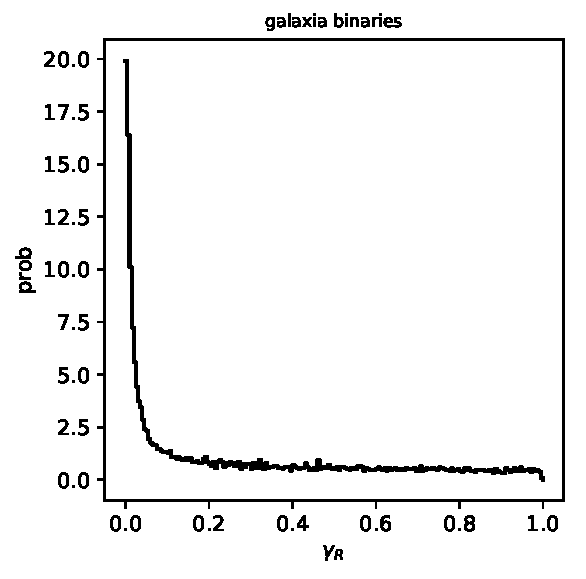
\includegraphics[scale=.8]{figures/galaxia_gammaR_distribn_mag_limited.pdf}
	\end{center}
	\caption{Light ratio distribution for the $r<17$ Galaxia sample discussed 
	in Sec.~\ref{subsec:introduce_binaries}.}
	\label{fig:galaxia_gammar_distribn}
\end{figure}
\begin{figure}[!t]
	\begin{center}
		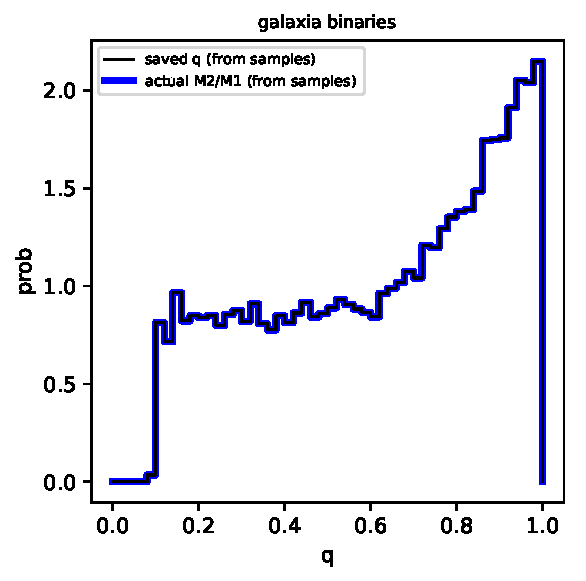
\includegraphics[scale=.8]{figures/galaxia_q_distribn_mag_limited.pdf}
	\end{center}
	\caption{Mass ratio distribution for the $r<17$ Galaxia sample discussed 
		in Sec.~\ref{subsec:introduce_binaries}.}
	\label{fig:galaxia_q_distribn}
\end{figure}
\begin{figure}[!t]
	\begin{center}
		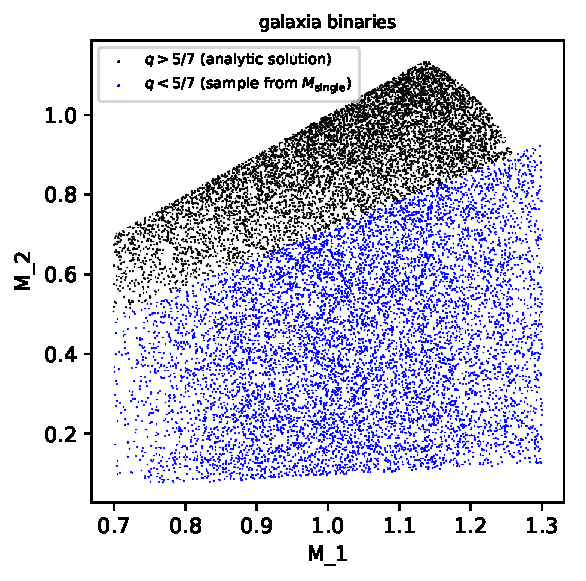
\includegraphics[scale=.8]{figures/galaxia_gammaR_scatter_masses.pdf}
	\end{center}
	\caption{Scatter plot of primary and secondary mass (solar units).}
	\label{fig:galaxia_scatter_masses}
\end{figure}
\begin{figure}[!t]
	\begin{center}
		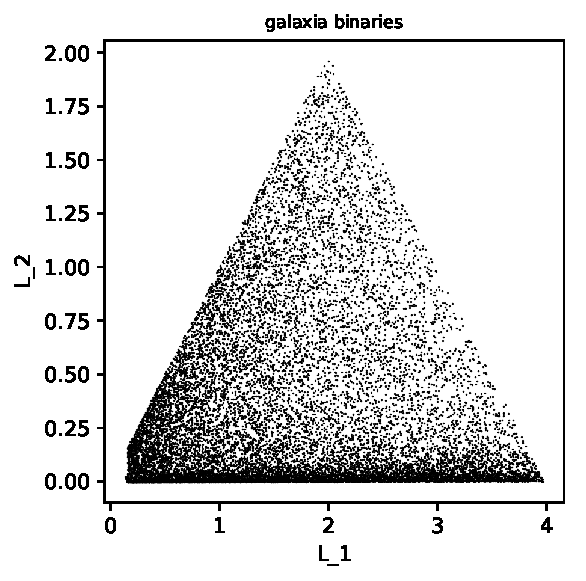
\includegraphics[scale=.8]{figures/galaxia_gammaR_scatter_luminosities.pdf}
	\end{center}
	\caption{Scatter plot of primary and secondary luminosity (solar units).}
	\label{fig:galaxia_scatter_luminosities}
\end{figure}
\begin{figure}[!t]
	\begin{center}
		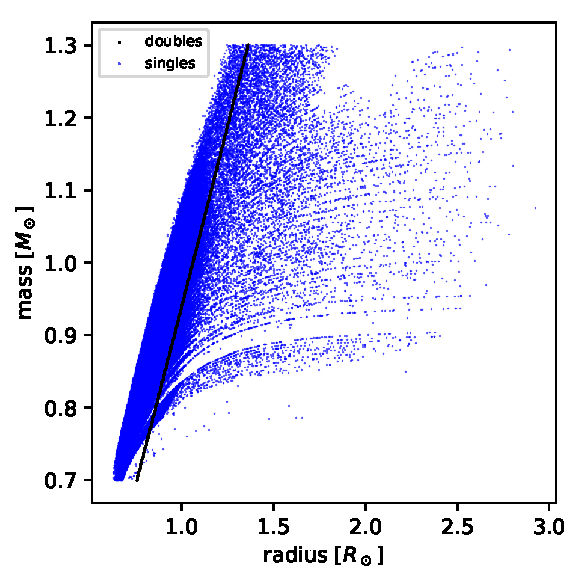
\includegraphics[scale=.8]{figures/galaxia_compare_mass_radius.pdf}
	\end{center}
	\caption{Scatter plot of mass vs radius for singles and binaries. For 
	binaries, different points are shown for the primary and secondary of a 
	given system. Only points with $0.7<M_\star/M_\odot<1.3$ are selected.}
	\label{fig:galaxia_mass_radius}
\end{figure}


\subsection{Using Galaxia to construct a KIC analog}

With glowing confidence, we then proceed to construct a KIC analog as follows.
We take all Galaxia stars within 7.5 degrees of the center of the \kepler\ 
field, and take stars with $r<17$.
\todo[inline]{a different magnitude cut, e.g. $r<16$, might matter?}
This is now beyond where the KIC is complete, so direct comparisons of 
distributions with the KIC will be confused.
We then apply an analog of the prioritization scheme used by the \kepler 
mission to select target stars, described by Batalha et al [2010]'s Table 1. 

For each star, we compute the minimum detectable planet radius at three 
semimajor axes: (1) the inner radius of the so-called ``habitable'' zone,
\begin{equation}
a_{\rm HZ} = 0.95\, {\rm AU} \left(\frac{L}{L_\odot}\right)^{1/2},
\end{equation}
(2) $0.5 a_{\rm HZ}$, and (3) $5R_\star$. We make the same assumptions as 
Batalha et al [2010] did about the transit duration. We assume a noise model of 
pure shot noise, rather than using any CDPP estimates.
We then apply the Batalha et al [2010] Table 1 prioritization, except 
that we use SDSS $r$ magnitudes instead of Kepler $Kp$ magnitudes.
The rankings are shown in Fig.~\ref{fig:batalha_table_1}.
We get similar (within a factor of two) counts as they did towards the end of 
the table, though at the beginning we seem to have fewer stars\footnote{I 
suspect this is because of the slightly different noise calculation -- and 
perhaps Batalha using $N_{\rm sample}$ rather than just counting photons 
matters}.

\begin{figure}
	\begin{center}
		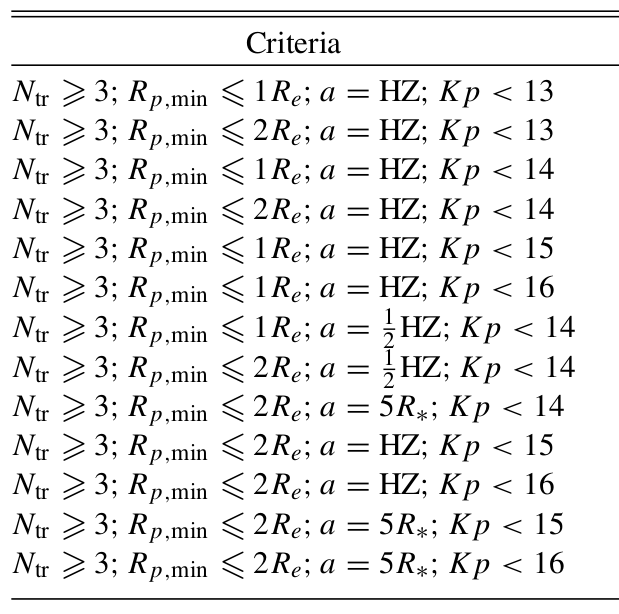
\includegraphics[scale=0.3]{figures/batalha_2010_table_1.png}
	\end{center}
	\caption{Prioritization applied by Batalha et al [2010], from whom I 
	copy-pasted this Table. I did the same, but using $r$ magnitudes instead of 
	$Kp$.}
	\label{fig:batalha_table_1}
\end{figure}
\begin{figure}[!t]
	\begin{center}
		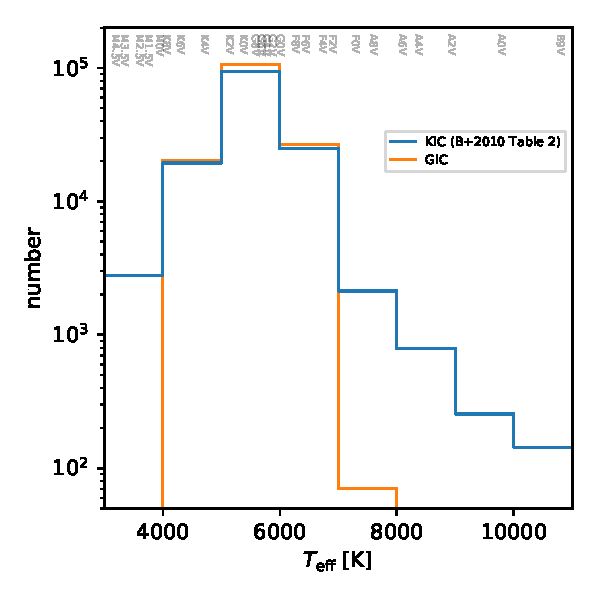
\includegraphics[scale=0.8]{figures/KIC_vs_GIC_teff_distribn.pdf}
	\end{center}
	\caption{Effective temperature distribution of the stars in our synthetic 
		Kepler input catalog analog -- the Galaxia input catalog.
		Note that the effective temperatures of binary star systems in the GIC 
		are 
		intentionally wrongly estimated, as if they were single star systems.
		The listed $T_{\rm eff}$ to spectral type correspondence is from 
		Mamajek's tables.
	}
	\label{fig:KIC_vs_GIC_teff_distribn}
\end{figure}


Note that, since we assigned binarity to Galaxia stars, applying the Batalha et 
al [2010] prioritization procedure requires estimating \textit{incorrect} 
single star parameters for what are really binary star systems!
We do this by keeping the total system luminosity, inverting 
Fig.~\ref{fig:mass_luminosity} to find an incorrect mass, and then applying 
Eq.~\ref{eq:mass_radius} to get an incorrect radius.
We can then calculate the minimum detectable planet radius as
\begin{equation}
R_{p,{\rm min}} = \left(\frac{7.1 \sigma_{\rm tot}}{r}\right)^{1/2} R_\star,
\label{eq:min_det_radius}
\end{equation}
for $r=1$ the dilution that we ignore, and
\begin{equation}
\sigma_{\rm tot} \equiv {\rm N} = (F_\gamma^{\rm N} A N_{\rm tra} T_{\rm 
dur})^{-1/2}
\end{equation}

In applying the prioritization, we omit the latter two priority classes of 
Fig.~\ref{fig:batalha_table_1}, to obtain a catalog of 152682 stellar systems, 
which we hereafter refer to as the \textit{Galaxia Input Catalog (GIC)}.
We compare the effective temperature distribution of the GIC with 
that of the KIC, reported by Batalha et al [2010] Table 2, in 
Fig.~\ref{fig:KIC_vs_GIC_teff_distribn}. Evidently, the GIC is 
dominated by sun-like stars, in a very similar manner to the exoplanet target 
stars of the KIC.


\subsection{Introduce a planet population}

As in Sec.~\ref{sec:model_2}, we allow for three different occurrence rates: 
$\Gamma_{t,s}$, the fraction of stars in single systems with a planet of radius 
$R_p$ and orbital period $P$, and also $\Gamma_{t,d1}$ and $\Gamma_{t,d2}$ for 
the fraction per sun-like primary and secondary (respectively) of double star 
systems with a planet of $(R_p, P)$.

We then randomly select which stars get a planet, and using the true stellar 
masses and radii compute the corresponding impact parameters for the planets as
\begin{equation}
b = \frac{a}{R_\star} \cos i, \quad \cos i \sim \mathcal{U}(0,1).
\end{equation}
Any planet with $|b| < 1$ is transiting, and has its transit duration evaluated 
as
\begin{equation}
T_{\rm dur} = 13\,{\rm hr} \left(\frac{P}{{\rm yr}}\right)^{1/3} 
\left(\frac{\rho_\star}{\rho_\odot}\right)^{-1/3} \sqrt{1 - b^2},
\end{equation}
which assumes circular orbits.

\subsection{Run the survey}
We run the following survey:
$A = 0.708\,{\rm m}^2$ (\kepler\ effective area), $T_{\rm obs} = 20\,{\rm 
years}$ (to detect more Earth-like planets than \kepler\ did), and $x_{\rm min} 
= 7.1$, the same signal to noise threshold as \kepler.

For simplicity, we assign a $r$ band zero point of $10^6\,{\rm ph/s/cm}^2$ to 
correspond to an $r=0$. We use this to compute the observed 
photon number fluxes for every system, regardless of whether it has a planet.
We then compute the signal to noise distribution of transit events, and the 
number of detections, according to Eq.~\ref{eq:snr_ivory_tower}.


\subsection{Numerically assess what occurrence rates would be derived, and 
	compare to previous models}

\subsubsection{If we ignore binarity, how wrong is our occurrence rate for 
	planets of radius $R_p$?}

This is similar to what we did in Sec.~\ref{subsubsec:model2_A}, with the 
exception that we need to specify the calculation more precisely.

Specifically, our ``Astronomer A'' in this case will estimate an occurrence 
rate for planets of radius $R_p$ and orbital period $P$ as
\begin{equation}
\Gamma_{{\rm A}, R_p} = \frac{N_{\rm det,s}}{Z},
\label{eq:rate_A}
\end{equation}
for
\begin{equation}
Z \approx (N_s + N_d) \frac{1}{J} \sum_{j=1}^{J} Q_j,
\end{equation}
for $Q_j$ the total detection efficiency, indexed over single and double 
systems, given as the product of the geometric transit probability and the 
system-specific completeness:
\begin{equation}
Q_j \equiv f_g^{(j)} f_c^{(j)}.
\end{equation}

Keep in mind that for Astronomer A, we need to compute the 
\textit{incorrect} transit probability for double star systems (since 
Astronomer A is assuming that they are single stars).

To evaluate the system-level completeness, we assume that Astronomer A performs 
something equivalent to perfect injection-recovery.
For a stellar system with known properties (stellar and planetary), and a 
perfectly known noise model, the probability of detection is a binary function: 
either ${\rm S/N} > {\rm (S/N)_{min}}$, or it is not\footnote{There are 
probabilities involved if we allow for any uncertainty in the parameters, but 
this is too complicated for our current goal.}.
So we compute $f_c^{(j)}$ as Astronomer A would: an array (over star systems) 
of zeros wherever the $(R_p,P)$ planet could not be detected, and ones where it 
could.
We then evaluate the total detection efficiency $Q_j$ for each system, and 
compute the occurrence rate as in Eq.~\ref{eq:rate_A}.
The resulting occurrence rates are only slightly smaller than those in 
Sec.~\ref{subsubsec:close_enough} discussed below and shown in 
Fig.~\ref{fig:error_vs_occrate}.

\subsubsection{What if we ignore binarity, but count planets whose derived 
radii are ``close enough'' to $R_p$?}
\label{subsubsec:close_enough}

As in Sec.~\ref{sec:model_2}, we now count planets with observed radii from 
$(1-x)R_\oplus < R_p^{\rm obs} < R_\oplus$. We'll use $x=0.1$, but it can be 
whatever we want.
The occurrence rate in this case will be
\begin{equation}
\Gamma_{A,R_p'} = \frac{N_{\rm det,s} + N_{\rm det,d}(R_p')}{Z'},
\end{equation}
for
\begin{equation}
Z' \approx (N_s + N_d) \frac{1}{J} \sum_{j=1}^{J} Q_j',
\end{equation}
where the geometric transit probability is the same as before, but the 
system-specific completeness is now a function of the desired radius interval:
\begin{equation}
Q_j' = f_g^{(j)} f_c^{(j)}(R_p').
\end{equation}
There are three possible cases for the completeness, specified by the minimum 
detectable planet radius $R_{p,{\rm min}}$ (computed according to 
Eq.~\ref{eq:min_det_radius}):
\begin{align}
f_c^{(j)}(R_p') &= 
\Bigg\{\begin{array}{lr}
1 & {\rm\ if\ }R_{p,{\rm min}}>R_p,\\
0, & {\rm\ if\ }R_{p,{\rm min}}<(1-x)R_p,\\
\frac{R_p - R_{p,{\rm min}}}{R_p - (1-x)R_p}, &{\rm otherwise}.
\end{array}
\label{eq:completeness_close_enough}
\end{align}
The latter term above is the case in which the minimum detectable planet 
radius happens to be between $(1-x)R_p$ and $R_p$. In that case the 
completeness becomes the fraction of planets in that interval that would be 
detected.
Assuming a uniform prior for the planet radius distribution $R_p \sim 
\mathcal{U}((1-x)R_p, R_p)$, this becomes the expression given in 
Eq.~\ref{eq:completeness_close_enough}.

These occurrence rates can then be compared to the ``true occurrence rate'' 
derived by the all-knowing Astronomer D:
\begin{equation}
\Gamma_{{\rm D}, R_p} = \frac{\Gamma_{t,s} N_s + (\Gamma_{t,d1} + 
						\Gamma_{t,d2})N_d}{N_s + 2 N_d}.
\end{equation}
A note in passing: the more information-rich parameters for Astronomer D to 
report would be $(\Gamma_{t,s}, \Gamma_{t,d1}, \Gamma_{t,d2})$, rather than 
$\Gamma_{{\rm D}, R_p}$. But I digress.

Similar to Fig.~\ref{fig:XGamma_vs_xi}, Fig.~\ref{fig:error_vs_occrate} 
shows that the magnitude of the relative error 
made by the $\Gamma_{{\rm A},R_p'}$ and $\Gamma_{{\rm A},R_p}$ estimates 
depends strongly 
on the fraction of secondaries that are assumed to host the $(R_p, P)$ planets.
The simplest assumption is that the occurrence rate is the same for all solar 
type stars: any ``Sun-like'' ($0.7<M_\star/M_\odot<1.3$) star hosts planets at 
the ``true rate'' $\Gamma_t$, and any other mass of star does not.
Given how we have defined the GIC, this means that all single stars and 
primaries of double star systems are sun-like. The fraction of Sun-like 
secondaries in this case is 37.4\% of all secondaries.
Reading the appropriate value off Fig.~\ref{fig:error_vs_occrate}, this 
corresponds to $\Gamma_{\rm D} = 1.39 \Gamma_{\rm A'}$.


\begin{figure}[!t]
	\begin{center}
		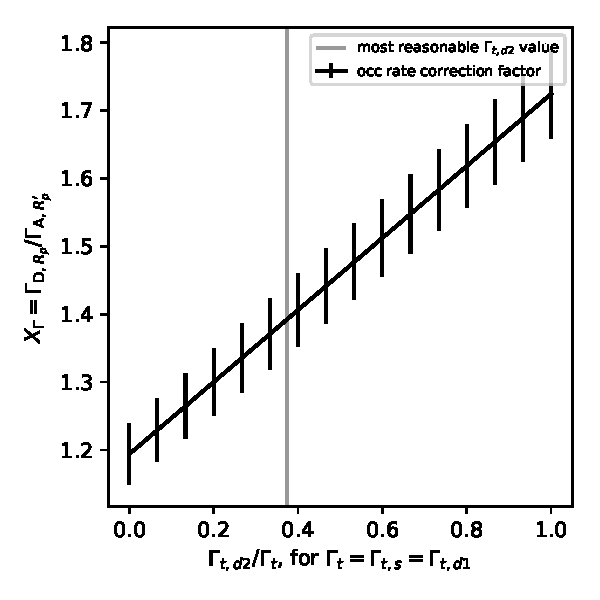
\includegraphics[scale=0.8]{figures/error_vs_occrate.pdf}
	\end{center}
	\caption{ The ``most reasonable'' $\Gamma_{t,d2}$ value is obtained by 
	assuming that the occurrence rate of $(R_p, P)$ planets is the same for all 
	solar type stars, and zero otherwise.
	This applies most immediately to the question of Earth-like planets around 
	Sun-like stars.
	}
	\label{fig:error_vs_occrate}
\end{figure}




% \begin{comment}
% \subsection{How many stars are in the sample?}
% \subsection{How many planets are in the sample?}
% \subsection{What is the true occurrence rate?}
% \subsection{How many planets are detected?}
% \subsubsection{Analytic completeness}
% \subsubsection{Deriving ${\rm prob}(x_i)$}
% \subsubsection{Number of detected planets}
% \subsection{Astronomer A ignores binarity}
% \subsection{Astronomer B counts host stars correctly}
% \subsection{Astronomer C counts host stars correctly and figures out diluted
% radii}
% \subsection{Astronomer D counts host stars correctly, figures out diluted
% radii, and accounts for completeness}
% \subsection{Numerical verification}
% \subsection{Representative numbers for a few cases}
% \subsubsection{If we ignore binarity, for what fraction of detections do we
% misclassify the radii?}
% \subsubsection{If we ignore binarity, how wrong is our occurrence rate for
% planets of radius $R_p$?}
% \subsubsection{If we ignore binarity, but allow derived planet radii to be
% ``close enough'', how do we do?}
% 
% \end{comment}


\newpage

%\begin{thebibliography}{}


%\end{thebibliography}

\end{document}
